%% Elsevier single-column manuscript.
\documentclass[a4paper,fleqn]{cas-sc}

\usepackage[authoryear,longnamesfirst]{natbib}
\usepackage{amsmath}
\usepackage{amssymb}
\usepackage{array}
\usepackage{float}
\usepackage{placeins}
\usepackage{booktabs}
\usepackage{graphicx}
\usepackage{xcolor}

% Inlined rows use \csvcomma{} where literal commas are needed inside cells.
\newcommand{\rccite}[2]{\textcolor{blue}{[#1] #2}}
\newcommand{\csvcomma}{,}

%%% Author macros
\def\tsc#1{\csdef{#1}{\textsc{\lowercase{#1}}\xspace}}
\tsc{WGM}
\tsc{QE}

\ExplSyntaxOn
\keys_set:nn { stm / mktitle } { nologo }
\cs_set:Npn \__first_footerline:
{
    \group_begin:
    \small
    \sffamily
    \ifnum\theblind>0\relax
    \else
        \__short_authors:
    \fi
    \group_end:
}
\ExplSyntaxOff

\begin{document}
\let\WriteBookmarks\relax
\def\floatpagepagefraction{1}
\def\textpagefraction{.001}

\shorttitle{Mass Conservation and Non-Negativity in Activated Sludge Systems}
\shortauthors{}

\title[mode=title]{Enforcement of Mass Conservation and Non-Negativity in Statistical Surrogates of Activated Sludge Systems}

\author{}

\begin{abstract}
Fast statistical surrogates are useful in activated sludge modeling only if their predictions can still be treated as physically possible process states. This study tested whether a model-agnostic post-prediction projection could enforce two non-negotiable requirements--mass conservation and non-negative concentrations--after a surrogate has produced a complete 20-component effluent prediction. The Kircher--Votsmeier conservative projection was transferred to a steady-state activated sludge benchmark and evaluated with 13 surrogates: XGBoost, LightGBM, CatBoost, AdaBoost, Random Forest, Extra Trees, SVR, $k$-NN, PLS, Multi-task Elastic Net, Multi-task Lasso, MLP, and TabNet. These models were tested across eleven training-set sizes, nested in-distribution cross-validation, and two out-of-distribution regimes. Every raw surrogate prediction set violated mass conservation, and several accurate raw surrogates also predicted negative small components. After projection, all $766{,}350$ evaluated predictions conserved mass and remained non-negative, with maximum conservation residuals of $2.06\times10^{-13}$ in-distribution and $1.72\times10^{-13}$ out-of-distribution. Projection often helped accuracy, lowering about three quarters of component-level nRMSE comparisons and 20 of 26 out-of-distribution aggregate comparisons, but it did not improve every aggregate score. The central lesson is practical: physical admissibility and predictive accuracy are separate requirements, and projection supplies the former without retraining the surrogate.
\end{abstract}

\begin{highlights}
\item Fast activated sludge surrogates can be accurate but physically inadmissible.
\item Thirteen surrogates were tested across data scarcity and extrapolation regimes.
\item Every raw surrogate set violated mass conservation; several predicted negatives.
\item Projection made all $766{,}350$ predictions conserve mass and stay non-negative.
\item Accuracy gains varied, so feasibility and error must be evaluated separately.
\end{highlights}

\begin{keywords}
machine learning \sep wastewater treatment \sep activated sludge model \sep statistical surrogates \sep mass conservation \sep non-negativity
\end{keywords}

\maketitle

\section*{Nomenclature}
\noindent Only nonstandard mathematical variables, sets, and operators are listed; process abbreviations and component names are defined in the text.
\begin{tabbing}
\hspace{4.4cm} \= \kill
$A\in\mathbb{R}^{K\times F}$ \> Full-row-rank matrix of independent stoichiometric invariants \\
$b_i\in\mathbb{R}^{K}$ \> Conservation target for sample $i$\csvcomma{} $b_i=A c_{in\csvcomma{}i}$ \\
$c\in\mathbb{R}^{F}$ \> Generic ASM component-concentration vector \\
$c_{in\csvcomma{}i}\csvcomma{}c_{out\csvcomma{}i}\in\mathbb{R}^{F}$ \> Influent and true steady-state effluent vectors for sample $i$ \\
$c_{raw\csvcomma{}i}^{(m)}\csvcomma{}c_{+\csvcomma{}i}^{(m)}$ \> Raw prediction and positive provisional target \\
$c_{cand\csvcomma{}i}^{(m)}\csvcomma{}\tilde c_i^{(m)}$ \> Conservative candidate and final projected prediction \\
$D_i$ \> Hydraulic dilution rate\csvcomma{} $24\,\mathrm{h\,d}^{-1}/\mathrm{HRT}_i$ \\
$d_{c\csvcomma{}i}^{\mathrm{std}\csvcomma{}(m)}(\mathcal{T})$ \> Projection displacement standardized using reference set $\mathcal{T}$ \\
$e_{S_O}\in\mathbb{R}^{F}$ \> Unit vector selecting the dissolved-oxygen component \\
$F\csvcomma{}K\csvcomma{}P$ \> Numbers of ASM components\csvcomma{} invariants\csvcomma{} and processes; 20\csvcomma{} 5\csvcomma{} and 28 \\
$f_m:\mathbb{R}^{22}\to\mathbb{R}^{F}$ \> Trained statistical surrogate indexed by $m$ \\
$I_{comp}\in\mathbb{R}^{4\times F}$ \> Map from ASM components to COD\csvcomma{} TN\csvcomma{} TP\csvcomma{} and TSS \\
$\lambda_O\in\mathbb{R}^{P}$ \> Process-coordinate vector satisfying $\nu^\top\lambda_O=e_{S_O}$ \\
$N$ \> Total observations at a data-scarcity scale \\
$n\csvcomma{}n_\zeta$ \> Observations in one in-distribution validation fold and out-of-distribution regime $\zeta$ \\
$\mathcal{T}$ \> Designated training reference set: $\mathcal{T}_{N\csvcomma{}g}$ for in-distribution or $\mathcal{T}_{\mathrm{in\text{-}distribution}}$ for out-of-distribution \\
$q\csvcomma{}q_i^{*\csvcomma{}(m)}$ \> Arbitrary and optimal coordinates\csvcomma{} respectively\csvcomma{} in the basis $Z$ \\
$s_i^{(m)}$ \> Componentwise inverse of $c_{+\csvcomma{}i}^{(m)}$ \\
$u_i\in\mathbb{R}^{2}$ \> HRT and aeration variables for sample $i$ \\
$V_0\in\mathbb{R}^{F\times K}$ \> Matrix whose orthonormal columns span $\operatorname{null}(\nu)$ \\
$v_{mc\csvcomma{}i}(c)$ \> Mass-conservation residual of vector $c$ for sample $i$ \\
$v_{nn\csvcomma{}i}^{\mathrm{std}}(c;\mathcal{T})$ \> Negative magnitude of $c$ standardized using reference set $\mathcal{T}$ \\
$W_{s\csvcomma{}i}^{(m)}$ \> Diagonal relative-scaling matrix formed from $s_i^{(m)}$ \\
$x_i\in\mathbb{R}^{22}$ \> Concatenated operating and influent input for sample $i$ \\
$y\in\mathbb{R}^{4}$ \> Generic vector of the four reported effluent-quality composites \\
$Z\in\mathbb{R}^{F\times(F-K)}$ \> Matrix whose orthonormal columns span $\operatorname{null}(A)$ \\
$\alpha_i^{(m)}\csvcomma{}\delta_i^{(m)}$ \> Backtracking factor and conservative candidate direction \\
$\mathrm{nMSE}\csvcomma{}\mathrm{nRMSE}\csvcomma{}\mathrm{nMAE}$ \> Standardized error metrics defined in Equation~\eqref{eq:normalized_metrics} \\
$R^2\csvcomma{}\bar R^2$ \> Component and equal-weight macro-average coefficients of determination \\
$\Delta\mathrm{nRMSE}_{m\csvcomma{}N\csvcomma{}g}$ \> Projected minus raw nRMSE for surrogate $m$\csvcomma{} size $N$\csvcomma{} and fold $g$ \\
$\epsilon_{\mathrm{mach}}$ \> Machine precision for double-precision arithmetic \\
$\boldsymbol{\varepsilon}_c$ \> Component floor vector; each entry is $10^{-8}$ in its native unit \\
$\eta$ \> Numerical safety margin in positivity backtracking; $10^{-12}$ \\
$\zeta$ \> Out-of-distribution severity regime\csvcomma{} mild or severe \\
$\nu\in\mathbb{R}^{P\times F}$ \> ASM2d-TSN stoichiometric (Petersen) matrix \\
$\rho_i\in\mathbb{R}^{P}$ \> Biological and chemical process-rate vector for sample $i$ \\
$\sigma_j^{(\mathcal{T})}\csvcomma{}\boldsymbol{\sigma}^{(\mathcal{T})}$ \> Component SD and SD vector estimated from training reference set $\mathcal{T}$ \\
$\tau_{mc}\csvcomma{}\boldsymbol{\tau}_{nn}$ \> Conservation and componentwise non-negativity tolerances \\
$\omega_i$ \> Net dissolved-oxygen transfer rate due to aeration \\
$\xi_{ij}^{(m\csvcomma{}t\csvcomma{}N\csvcomma{}g)}\csvcomma{}\xi_{ij}^{(m\csvcomma{}t\csvcomma{}\zeta)}$ \> Standardized residual in an in-distribution fold or out-of-distribution regime \\
$\pi_{mc}\csvcomma{}\pi_{nn}$ \> Conservation and non-negativity violation frequencies with context indices \\
$\mathcal{F}_i$ \> Conservative\csvcomma{} non-negative feasible set for sample $i$ \\
$\mathbb{1}[\cdot]$ \> Indicator function\csvcomma{} equal to one when its condition is true \\
$\oslash$ \> Elementwise division \\
$i\csvcomma{}j\csvcomma{}h\csvcomma{}p$ \> Sample\csvcomma{} component\csvcomma{} invariant-row\csvcomma{} and process indices \\
$m\csvcomma{}t\csvcomma{}\ell\csvcomma{}g$ \> Surrogate\csvcomma{} prediction-type\csvcomma{} input-feature\csvcomma{} and fold indices \\
$\zeta$ \> Out-of-distribution-regime index \\
\end{tabbing}

\section{Introduction}

Water pollution remains a major ecological and public-health challenge whose effects depend on pollutant sources, exposure pathways, and the vulnerability of affected populations (Lin et al., 2022; Madhav et al., 2019). Activated sludge processes address this burden through interacting biological and physicochemical transformations. Nitrogen removal alone involves multiple microbial groups and pathways whose contributions change with operating conditions (Duan et al., 2022). Activated sludge models represent these interactions mechanistically and provide a basis for tracking carbon, nitrogen, phosphorus, alkalinity, and solids in wastewater treatment systems (Henze et al., 2006). Their detail is valuable, but repeated simulation can become burdensome when the same model must be called many times for design exploration, sensitivity analysis, optimization, or operational screening. Wastewater-network and plant-design studies illustrate the scale of such decision problems, which can involve nonlinear process behavior, competing objectives, sustainability criteria, and many candidate configurations (Aboagye et al., 2021; Padron-Paez et al., 2020).

Statistical surrogates offer a practical way to make these evaluations faster. The review of Bhosekar \& Ierapetritou (2018) describes the use of surrogates in feasibility analysis and optimization, while emphasizing sampling, surrogate selection, and validation. In wastewater applications, Durkin et al. (2024) trained surrogates on high-fidelity simulations and embedded them in resource-recovery optimization, while Mao et al. (2024) used artificial-intelligence tools to balance effluent quality and aeration energy. Other recent studies have linked machine learning to operational decision support, waste-sludge prediction, and interpretable effluent-nitrogen prediction (Wang et al., 2025; Yang et al., 2025; Xiao et al., 2025). These examples show why statistical surrogates are attractive: a sufficiently accurate surrogate can evaluate many operating or design alternatives at a fraction of the cost of repeated mechanistic simulation.

The difficulty is that accuracy is not the only condition for a usable activated sludge state. Activated sludge reactors are governed by component mass balances, and their concentrations must remain non-negative (Araujo et al., 2013; Henze et al., 2006). A statistical surrogate can therefore be close to a mechanistic target in an error metric while still violating a declared conservation balance or predicting an impossible negative concentration. This is not only a wastewater concern. Studies of constrained machine learning show that models can achieve low prediction error while violating conservation laws, and that enforcing positivity or conservation usually requires explicit architectural, training, or post-processing mechanisms (Hansen et al., 2024; Kashinath et al., 2021; Kircher \& Votsmeier, 2025; Sturm \& Wexler, 2022). For wastewater decision support, such violations matter because surrogate outputs may be interpreted directly or passed into downstream optimization and control workflows.

Prior work has pursued physical constraint enforcement in several ways. Physics-informed approaches incorporate governing relations into training, but soft penalties encourage rather than guarantee enforcement for every prediction (Raissi et al., 2019; Min et al., 2024). Stronger approaches use specialized architectures, analytic constraints, probabilistic reconciliation, dimensionality reduction, or differentiable hard-enforcement layers (Beucler et al., 2021; Hansen et al., 2024; Min et al., 2024; Sturm et al., 2023; Sturm \& Wexler, 2020, 2022; Utkarsh et al., 2025). These studies demonstrate that physical structure can be built into learning systems, but they also leave a practical gap for wastewater surrogates: methods that enforce mass conservation do not necessarily enforce non-negativity, methods that enforce non-negativity can disturb conservation, and many solutions are tied to particular surrogate structures.

Kircher and Votsmeier (2025) addressed simultaneous mass-conservation and non-negativity enforcement through a projection applied after prediction. Their method enforces atom balance while preserving non-negative concentrations, and it was demonstrated for atmospheric chemistry, heterogeneous catalysis, and synthetic reaction systems. Because the projection is applied after a completed prediction is produced, it can in principle be used with different underlying surrogates without redesigning or retraining them. That property is attractive for activated sludge applications, where linear, kernel, neighbor, tree-ensemble, boosting, and neural-network surrogates may all be considered for the same prediction task.

The remaining question is whether this common post-prediction procedure transfers reliably to activated sludge effluent prediction. Existing wastewater studies do not provide a systematic cross-surrogate evaluation of simultaneous hard enforcement of mass conservation and non-negativity, and evidence from other scientific domains does not establish how such enforcement affects activated sludge prediction accuracy, data-scarcity behavior, computation, or extrapolation. This study addresses that gap by transferring the Kircher--Votsmeier projection to a simulated steady-state activated sludge benchmark and evaluating it across 13 statistical surrogates. The work asks whether one model-agnostic projection can consistently enforce both physical requirements across diverse predictors, and how that enforcement changes predictive performance within and beyond the training range. In doing so, the study separates physical admissibility from the empirical accuracy of the underlying statistical surrogates.

\section{Methods}

The methodological process was designed to test physical admissibility separately from ordinary predictive accuracy (Figure~\ref{fig:evaluation_workflow}). First, a steady-state ASM2d-TSN benchmark was generated and screened so that the reference effluent states occupied the intended activated sludge component domain. Second, the stoichiometric invariant operator was constructed to express the sample-specific mass-conservation equality and non-negative feasible set. Third, 13 statistical surrogates were trained under nested in-distribution cross-validation, with preprocessing and hyperparameter selection confined to the appropriate training folds. Fourth, every raw 20-component prediction was scored as produced and then passed through the Kircher--Votsmeier projection, allowing paired raw/projected comparisons of accuracy, mass conservation, non-negativity, correction size, computation, and out-of-distribution behavior.

\begin{figure}[!htbp]
\centering
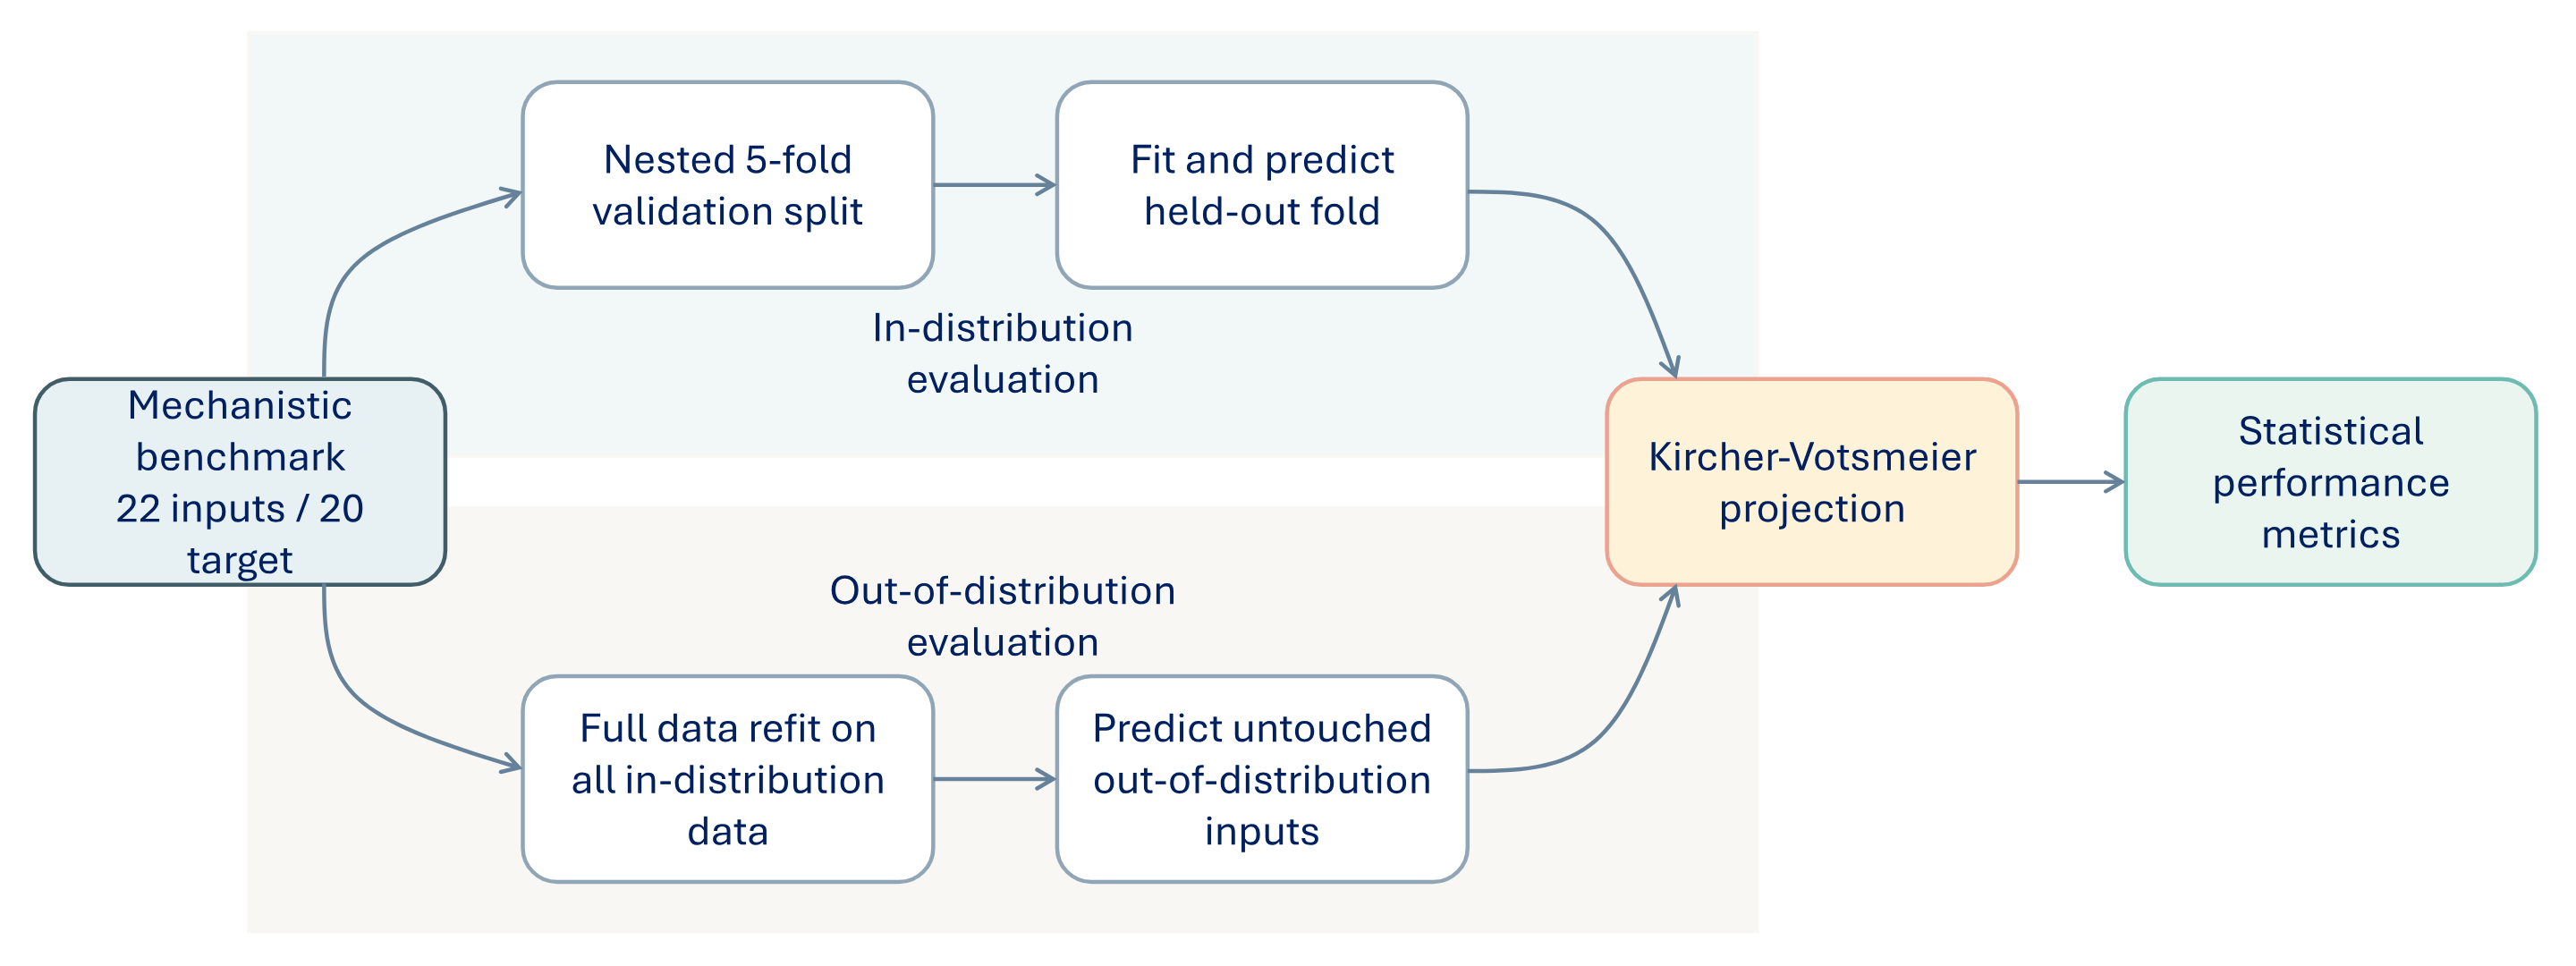
\includegraphics[width=\textwidth]{main_figure_evaluation_workflow.png}
\caption{Evaluation workflow linking nested in-distribution cross-validation, paired raw/projected scoring, and external out-of-distribution validation.}
\label{fig:evaluation_workflow}
\end{figure}
\FloatBarrier

\subsection{Simulated Activated Sludge Process and Dataset Generation}

The in-distribution benchmark data were generated with a standalone, steady-state continuous stirred tank reactor (CSTR). The reactor was represented by Activated Sludge Model No.\ 2d with two-step nitrification (ASM2d-TSN). This model contains 20 components and 28 coupled processes spanning hydrolysis, heterotrophic and phosphate-accumulating-organism metabolism, two-step nitrification and denitrification, lysis, and precipitation--redissolution. The model basis follows Henze et al. (2006), while the two-step nitrification formulation, stoichiometry, and rate coefficients follow Guerrero et al. (2011).

The dissolved components are dissolved oxygen ($S_O$), fermentable substrate ($S_F$), acetate ($S_A$), ammonium nitrogen ($S_{NH4}$), nitrite nitrogen ($S_{NO2}$), nitrate nitrogen ($S_{NO3}$), dinitrogen ($S_{N2}$), soluble phosphate ($S_{PO4}$), soluble inert organic matter ($S_I$), and alkalinity ($S_{ALK}$). The particulate components are particulate inert organic matter ($X_I$), slowly biodegradable substrate ($X_S$), heterotrophic biomass ($X_H$), phosphate-accumulating-organism biomass ($X_{PAO}$), stored polyphosphate ($X_{PP}$), stored polyhydroxyalkanoates ($X_{PHA}$), ammonia-oxidizing biomass ($X_{AOB}$), nitrite-oxidizing biomass ($X_{NOB}$), precipitated metal phosphate ($X_{MeP}$), and metal hydroxide ($X_{MeOH}$).

Every evaluated surrogate produces this same 20-component effluent state. For any component vector $c$, the reported vector is defined by
$y=(\mathrm{COD},\mathrm{TN},\mathrm{TP},\mathrm{TSS})^\top=I_{comp}c$,
where $I_{comp}\in\mathbb{R}^{4\times F}$ contains the fixed component-to-composite coefficients in that row order and the component order listed above. The full coefficients and their unit conversions are supplied with the benchmark data. This same map is applied to raw and projected predictions; the surrogates are not fitted directly to the four composites.

The simulation design sampled 22 continuous inputs: hydraulic retention time (HRT), aeration, and the 20 influent component concentrations. One randomized, scrambled strength-1 Latin hypercube with seed 42 and no post-optimization was linearly scaled to the bounds in Table~\ref{tab:simulation_domain}. All 10,000 candidates met the steady-state acceptance criterion and were retained. The tabulated intervals are sampling-design bounds rather than observed sample extrema; no input was held fixed.

\begin{table}[htbp]
\centering
\caption{Sampled operating and influent variables used to generate the steady-state Activated Sludge Model No.\ 2d with two-step nitrification (ASM2d-TSN) dataset.}
\label{tab:simulation_domain}
\scriptsize
\setlength{\tabcolsep}{3pt}
\begin{tabular}{p{2.1cm}p{2.7cm}p{2.8cm}p{3.0cm}}
\hline
Variable & Category & Range & Unit \\
\hline
$\mathrm{HRT}$ & Operating & [6.0\csvcomma{} 36.0] & h \\
$u_{\mathrm{air}}$ & Operating & [0.5\csvcomma{} 2.5] & -- \\
$S_O$ & Influent dissolved & [0.0\csvcomma{} 0.5] & g O$_2$/m$^3$ \\
$S_F$ & Influent dissolved & [20.0\csvcomma{} 180.0] & g COD/m$^3$ \\
$S_A$ & Influent dissolved & [5.0\csvcomma{} 80.0] & g COD/m$^3$ \\
$S_{NH4}$ & Influent dissolved & [12.0\csvcomma{} 55.0] & g N/m$^3$ \\
$S_{NO2}$ & Influent dissolved & [0.0\csvcomma{} 3.0] & g N/m$^3$ \\
$S_{NO3}$ & Influent dissolved & [0.0\csvcomma{} 8.0] & g N/m$^3$ \\
$S_{N2}$ & Influent dissolved & [0.0\csvcomma{} 2.0] & g N/m$^3$ \\
$S_{PO4}$ & Influent dissolved & [2.0\csvcomma{} 18.0] & g P/m$^3$ \\
$S_I$ & Influent dissolved & [10.0\csvcomma{} 90.0] & g COD/m$^3$ \\
$S_{ALK}$ & Influent dissolved & [80.0\csvcomma{} 260.0] & mol/m$^3$ \\
$X_I$ & Influent particulate & [20.0\csvcomma{} 120.0] & g COD/m$^3$ \\
$X_S$ & Influent particulate & [60.0\csvcomma{} 280.0] & g COD/m$^3$ \\
$X_H$ & Influent particulate & [15.0\csvcomma{} 100.0] & g COD/m$^3$ \\
$X_{PAO}$ & Influent particulate & [5.0\csvcomma{} 60.0] & g COD/m$^3$ \\
$X_{PP}$ & Influent particulate & [2.0\csvcomma{} 20.0] & g P/m$^3$ \\
$X_{PHA}$ & Influent particulate & [1.0\csvcomma{} 30.0] & g COD/m$^3$ \\
$X_{AOB}$ & Influent particulate & [0.5\csvcomma{} 8.0] & g COD/m$^3$ \\
$X_{NOB}$ & Influent particulate & [0.5\csvcomma{} 8.0] & g COD/m$^3$ \\
$X_{MeP}$ & Influent particulate & [0.0\csvcomma{} 12.0] & g TSS/m$^3$ \\
$X_{MeOH}$ & Influent particulate & [0.0\csvcomma{} 12.0] & g TSS/m$^3$ \\
\hline
\end{tabular}
\end{table}

For each sampled input, nonlinear least squares solved the steady-state balance equations under componentwise numerical state bounds of $10^{-8}$ and 1500, interpreted in each component's native unit from Table~\ref{tab:simulation_domain}. The solver's cost-change, step-size, and gradient convergence tolerances were each $10^{-9}$, and each solve was limited to 1200 function evaluations. Candidate generation used a global cap equal to 25 times the target retained-row count. Two physically informed initializations were tried first. If both failed, the process was dynamically relaxed for 20 days with a stiff backward differentiation formula (BDF) integrator, and its terminal state became a new steady-state guess. The balance-residual coordinates retain their corresponding native component-unit-per-day scales; only converged states with maximum absolute numerical residual no greater than $10^{-9}$ were retained. The 28 mechanistic process rates were evaluated from the ASM2d-TSN kinetics without an artificial rate ceiling or rate clipping; the stated bounds apply to solved state variables, not to reaction rates.

\begin{table}[htbp]
\centering
\caption{Simulation and acceptance settings used to construct the benchmark dataset.}
\label{tab:simulation_settings}
\scriptsize
\begin{tabular}{p{3.7cm}p{7.2cm}}
\hline
Setting & Value or rule \\
\hline
Process model & Standalone steady-state continuous stirred tank reactor based on ASM2d-TSN \\
ASM components & 20 effluent component targets and 20 influent component references \\
Reaction processes & 28 coupled biological and chemical processes \\
Process-rate handling & Mechanistic rates evaluated directly; no artificial clipping or rate ceiling \\
Reported composites & COD\csvcomma{} TN\csvcomma{} TP\csvcomma{} and TSS computed with $I_{comp}$ \\
Sampling design & Latin hypercube sampling over 22 inputs \\
Random seed & 42 \\
Accepted samples & 10\csvcomma{}000 converged steady states \\
Steady-state solver & Nonlinear least squares under box constraints \\
State bounds & $[10^{-8}\csvcomma{}1500]$ during the steady-state solve \\
Solver tolerances & Variable\csvcomma{} residual\csvcomma{} and gradient tolerances of $10^{-9}$ \\
Function evaluations & Maximum of 1200 per nonlinear solve \\
Candidate attempts & Global cap of 25 times the target retained-row count \\
Fallback initialization & 20-day stiff backward differentiation formula dynamic relaxation if two steady-state initializations fail \\
Acceptance criterion & Maximum absolute residual no greater than $10^{-9}$ \\
\hline
\end{tabular}
\end{table}

The first initialization blended the current influent state with the previous accepted effluent state when such a previous state was available, adjusted readily consumed substrates downward, preserved biomass pools, and estimated dissolved oxygen from hydraulic dilution and oxygen-transfer terms. The multistart initialization reused the primary state but applied stronger substrate depletion and biomass enrichment. Both candidate initial states were clipped to $[10^{-6},1500]$ before solving. This clipping applies only to starting state vectors; the mechanistic process rates themselves are not clipped. These initialization rules were used only to obtain converged process-model samples; they were not used as features in the surrogates.

\subsection{Mass-Conservation Invariants and Non-Negative Feasible Component Space}

Let $c_{in,i},c_{out,i}\in\mathbb{R}^{F}$ denote the influent and effluent component vectors for sample $i$, and let $\nu\in\mathbb{R}^{P\times F}$ be the ASM2d-TSN Petersen matrix, with $P=28$ and $F=20$. Numerical rank is the number of singular values exceeding the standard threshold $\max(P,F)\epsilon_{\mathrm{mach}}\|\nu\|_2=28\,\epsilon_{\mathrm{mach}}\|\nu\|_2$, where $\|\nu\|_2$ is the largest singular value of $\nu$. This calculation gives $\operatorname{rank}(\nu)=15$ and hence, by the rank--nullity relation, a right-null-space dimension of $K=F-15=5$. Let the columns of $V_0\in\mathbb{R}^{F\times K}$ be the orthonormal basis for that right null space, so $\nu V_0=\mathbf{0}_{P\times K}$. Defining $A=V_0^\top\in\mathbb{R}^{K\times F}$ then gives
\begin{equation}
\label{eq:invariant_operator}
A\nu^\top=V_0^\top\nu^\top=(\nu V_0)^\top=\mathbf{0}_{K\times P},
\qquad
AA^\top=V_0^\top V_0=I_K.
\end{equation}
This construction makes each row of $A$ an independent linear combination of components that reactions cannot change. For the adopted steady-state system boundary, the component balance for sample $i$ is
\begin{equation}
\label{eq:steady_component_balance}
D_i(c_{out,i}-c_{in,i})=\nu^\top\rho_i+\omega_i e_{S_O},
\end{equation}
where $D_i>0$ is the hydraulic dilution rate, $\rho_i\in\mathbb{R}^{P}$ contains the biological and chemical process rates evaluated at $c_{out,i}$, and $\omega_i e_{S_O}$ is the external dissolved-oxygen transfer caused by aeration. With HRT entered in hours and the dimensionless aeration coordinate denoted by $u_{\mathrm{air},i}$, the simulator uses
\begin{equation}
D_i=\frac{24\,\mathrm{h\,d}^{-1}}{\mathrm{HRT}_i},\qquad
k_{La,i}=(2+18u_{\mathrm{air},i})\ {\rm d}^{-1},\qquad
\omega_i=k_{La,i}\!\left(S_{O,\mathrm{sat}}-e_{S_O}^\top c_{out,i}\right),
\end{equation}
where $S_{O,\mathrm{sat}}=8.5$ g O$_2$/m$^3$. Each component in these vector equations is represented by its numerical value in the fixed native unit listed in Table~\ref{tab:simulation_domain}. Premultiplication of Equation~\eqref{eq:steady_component_balance} by $A$ gives
\begin{equation}
\label{eq:invariant_balance}
D_iA(c_{out,i}-c_{in,i})
=\underbrace{A\nu^\top}_{\mathbf{0}_{K\times P}}\rho_i+\omega_iAe_{S_O}.
\end{equation}
Thus, Equation~\eqref{eq:invariant_operator} eliminates every biological and chemical reaction contribution, irrespective of the values in $\rho_i$. The same rank calculation gives $e_{S_O}\in\operatorname{range}(\nu^\top)$, so there exists $\lambda_O\in\mathbb{R}^{P}$ such that
\begin{equation}
Ae_{S_O}=A\nu^\top\lambda_O=\mathbf{0}_K.
\end{equation}
In exact arithmetic, this relation and $D_i>0$ reduce Equation~\eqref{eq:invariant_balance} to $Ac_{out,i}=Ac_{in,i}$. The stored double-precision basis gives $\max_h|(Ae_{S_O})_h|=1.10\times10^{-13}$, below the numerical-rank threshold $1.55\times10^{-13}$ and consistent with roundoff. No balance-error bound is inferred from that coefficient alone. Mechanistic states were accepted by the steady-state residual criterion in Table~\ref{tab:simulation_settings}; their observed invariant residuals and minimum components are reported separately in the Results. This motivates the sample-specific target and feasible effluent set
\begin{equation}
\label{eq:feasible_set}
b_i:=A c_{in,i},\qquad
\mathcal{F}_i:=\left\{c\in\mathbb{R}^{F}:Ac=b_i,\ c\geq\mathbf{0}\right\}.
\end{equation}
The equality in Equation~\eqref{eq:feasible_set} is therefore the resolved boundary balance, while $c\geq\mathbf{0}$ adds componentwise non-negativity. Because the sampled influent satisfies $c_{in,i}\geq\mathbf{0}$, it belongs to $\mathcal{F}_i$ and provides a feasible anchor for the projection. All accepted mechanistic states were componentwise positive. Their finite-precision invariant residuals were evaluated separately and are reported in the Results; mechanistic-state acceptance used the maximum steady-state balance residual of $10^{-9}$ specified in Table~\ref{tab:simulation_settings}.

Table~\ref{tab:invariant_matrix} reports the numerical basis in the fixed target order. Coefficients are displayed to six decimal places for readability, whereas all calculations retain double precision. No row-wise renormalization or coefficient rounding is applied before projection. With the unrounded basis, the maximum absolute entry of $A\nu^\top$ is $4.25\times10^{-16}$. Any nonsingular row transformation of $A$ defines the same feasible equality, but all reported residual magnitudes use the stored, unrounded orthonormal basis shown here. The row labels therefore identify basis vectors rather than separately named elemental balances. Throughout this article, ``mass conservation'' denotes satisfaction of these five stoichiometric invariants for the stated steady-state system boundary; it does not establish every possible elemental, kinetic, or plant-wide balance.

\begin{table}[htbp]
\centering
\caption{Invariant operator $A$ in the 20-component ASM2d-TSN target order. Displayed coefficients are rounded; the unrounded orthonormal basis is used in all calculations.}
\label{tab:invariant_matrix}
\scriptsize
\resizebox{\textwidth}{!}{%
\begin{tabular}{lrrrrrrrrrr}
\toprule
 & $S_O$ & $S_F$ & $S_A$ & $S_{NH4}$ & $S_{NO2}$ & $S_{NO3}$ & $S_{N2}$ & $S_{PO4}$ & $S_I$ & $S_{ALK}$ \\
\midrule
$a_1^\top$ & 0 & 0 & 0 & -0.493398 & -0.499144 & -0.499144 & -0.496271 & -0.016018 & 0.031680 & -0.040218 \\
$a_2^\top$ & 0 & 0 & 0 & -0.033427 & -0.009065 & -0.009065 & -0.021246 & 0.683584 & -0.113953 & 0.170531 \\
$a_3^\top$ & 0 & 0 & 0 & -0.015560 & 0.038009 & 0.038009 & 0.011224 & 0.018519 & 0.822862 & 0.374985 \\
$a_4^\top$ & 0 & 0 & 0 & 0.108417 & -0.019450 & -0.019450 & 0.044483 & 0.150345 & 0.258480 & -0.895071 \\
$a_5^\top$ & 0 & 0 & 0 & -0.006905 & -0.023309 & -0.023309 & -0.015107 & 0.049396 & 0.492034 & -0.114822 \\
\midrule
 & $X_I$ & $X_S$ & $X_H$ & $X_{PAO}$ & $X_{PP}$ & $X_{PHA}$ & $X_{AOB}$ & $X_{NOB}$ & $X_{MeP}$ & $X_{MeOH}$ \\
\midrule
$a_1^\top$ & -0.010099 & 0 & -0.035085 & -0.035085 & -0.017315 & 0 & -0.035085 & -0.035085 & 0.033138 & 0.051796 \\
$a_2^\top$ & 0.006466 & 0 & 0.012294 & 0.012294 & 0.689085 & 0 & 0.012294 & 0.012294 & 0.088467 & -0.074856 \\
$a_3^\top$ & 0.000531 & 0 & 0.001398 & 0.001398 & 0.030615 & 0 & 0.001398 & 0.001398 & 0.247874 & 0.341024 \\
$a_4^\top$ & 0.002104 & 0 & 0.005543 & 0.005543 & 0.121472 & 0 & 0.005543 & 0.005543 & 0.179747 & 0.218521 \\
$a_5^\top$ & 0.000155 & 0 & -0.000144 & -0.000144 & 0.045692 & 0 & -0.000144 & -0.000144 & -0.490609 & -0.705784 \\
\bottomrule
\end{tabular}}
\end{table}

\subsection{Kircher--Votsmeier Post-Prediction Projection}

The positivity-preserving conservative projection of Kircher and Votsmeier (2025) is applied after prediction and does not alter the underlying surrogate. The projection has three stages: construct a positive provisional state, project its change into the conservation-preserving subspace, and shorten that conservative change only when needed to ensure non-negativity. With $u_i\in\mathbb{R}^{2}$ containing HRT and aeration, the complete input is the column vector $x_i=[u_i^\top,c_{in,i}^\top]^\top\in\mathbb{R}^{22}$. A trained surrogate $f_m:\mathbb{R}^{22}\rightarrow\mathbb{R}^{F}$ first produces the finite vector
\begin{equation}
\label{eq:raw_component_prediction}
c_{raw,i}^{(m)}=f_m(x_i).
\end{equation}
The projection then constructs a strictly positive provisional target and its relative-error weights,
\begin{equation}
\label{eq:positive_scaling}
c_{+,i}^{(m)}=\max\!\left(c_{raw,i}^{(m)},\boldsymbol{\varepsilon}_c\right),\qquad
s_i^{(m)}=\mathbf{1}\oslash c_{+,i}^{(m)},\qquad
W_{s,i}^{(m)}=\operatorname{Diag}\!\left(s_i^{(m)}\right),
\end{equation}
where the maximum and division are componentwise. Each entry of the floor vector $\boldsymbol{\varepsilon}_c$ is $10^{-8}$ in the native unit of its component. The lower-bounded vector $c_{+,i}^{(m)}$ supplies both the target change in Equation~\eqref{eq:kv_scaled_projection} and its weights; it is not reported as a clipped prediction. Multiplication by $W_{s,i}^{(m)}$ converts each projection residual to a relative residual, so near-zero components receive larger weights.

Let $Z\in\mathbb{R}^{F\times(F-K)}$ have orthonormal columns spanning $\operatorname{null}(A)$, so $AZ=\mathbf{0}_{K\times(F-K)}$ and $Z^\top Z=I_{F-K}$. Because $Ac_{in,i}=b_i$, every vector in the conservation affine space can be written as
\begin{equation}
\label{eq:conservative_parameterization}
\{c:Ac=b_i\}
=\{c_{in,i}+Zq:q\in\mathbb{R}^{F-K}\}.
\end{equation}
The projection therefore selects the conservative change $Zq$ that is closest, in the relative scaling of Equation~\eqref{eq:positive_scaling}, to the provisional change $c_{+,i}^{(m)}-c_{in,i}$:
\begin{equation}
\label{eq:kv_scaled_projection}
q_i^{*,(m)}=\underset{q\in\mathbb{R}^{F-K}}{\operatorname{argmin}}\;
\left\|W_{s,i}^{(m)}\left[Zq-\left(c_{+,i}^{(m)}-c_{in,i}\right)\right]\right\|_2,
\end{equation}
The minimizer follows by setting the gradient of the squared objective to zero:
\begin{equation}
\label{eq:kv_optimality}
\left[Z^\top\!\left(W_{s,i}^{(m)}\right)^2Z\right]q_i^{*,(m)}
=Z^\top\!\left(W_{s,i}^{(m)}\right)^2
\left(c_{+,i}^{(m)}-c_{in,i}\right).
\end{equation}
Because $W_{s,i}^{(m)}$ has a strictly positive diagonal and $Z$ has full column rank, this system has a unique solution. Substitution into the affine parameterization gives the initial conservative candidate
\begin{equation}
\label{eq:conservative_candidate}
c_{cand,i}^{(m)}=c_{in,i}+Zq_i^{*,(m)}.
\end{equation}
Indeed, $Ac_{cand,i}^{(m)}=Ac_{in,i}+AZq_i^{*,(m)}=b_i$, which proves conservation before backtracking. Numerically, Equation~\eqref{eq:kv_scaled_projection} is solved from $W_{s,i}^{(m)}Z$ by an orthogonal--triangular factorization; singular-value decomposition with a relative cutoff of $10^{-12}$ is the fallback, and no normal-equation inverse is formed. If $Ac_{+,i}^{(m)}=b_i$, then $c_{+,i}^{(m)}-c_{in,i}\in\operatorname{null}(A)$, the least-squares residual can be zero, and the candidate equals $c_{+,i}^{(m)}$ to numerical tolerance.

Scaling protects trace components but does not alone prove non-negativity for an arbitrary raw vector. Define the conservative direction $\delta_i^{(m)}=c_{cand,i}^{(m)}-c_{in,i}=Zq_i^{*,(m)}$ and consider the line $c_{in,i}+\alpha\delta_i^{(m)}$ for $0\leq\alpha\leq1$. For each component with $\delta_{ij}^{(m)}<0$, non-negativity requires
$c_{in,ij}+\alpha\delta_{ij}^{(m)}\geq0$, or equivalently
$\alpha\leq c_{in,ij}/(-\delta_{ij}^{(m)})$. Taking the most restrictive such bound and applying the safety margin $\eta=10^{-12}$ gives
\begin{equation}
\alpha_i^{(m)}=
\begin{cases}
1, & \min_j c_{cand,ij}^{(m)}\geq0,\\
(1-\eta)\displaystyle\min_{j:\delta_{ij}^{(m)}<0}
\frac{c_{in,ij}}{-\delta_{ij}^{(m)}}, & \text{otherwise},
\end{cases}
\qquad
\tilde c_i^{(m)}=c_{in,i}+\alpha_i^{(m)}\delta_i^{(m)}.
\label{eq:positivity_backtracking}
\end{equation}
In the second branch at least one ratio is below one, while non-negativity of $c_{in,i}$ makes every ratio non-negative; hence $0\leq\alpha_i^{(m)}<1$. For $\delta_{ij}^{(m)}<0$, the construction gives $\tilde c_{ij}^{(m)}\geq\eta c_{in,ij}\geq0$, and components with non-negative direction remain non-negative. The implementation clips $\alpha_i^{(m)}$ to $[0,1]$ against roundoff. Thus $\tilde c_i^{(m)}\geq\mathbf{0}$. It also preserves conservation because
\begin{equation}
A\tilde c_i^{(m)}
=Ac_{in,i}+\alpha_i^{(m)}AZq_i^{*,(m)}
=b_i.
\end{equation}
The implementation accepts a projection when $\|A\tilde c_i^{(m)}-b_i\|_2\leq\tau_{mc}$ and $\tilde c_{ij}^{(m)}\geq-\tau_{nn,j}$ for every component $j$. Here $\tau_{mc}=10^{-10}$ is the basis-specific invariant-residual tolerance and each entry of $\boldsymbol{\tau}_{nn}$ is $10^{-10}$ in its component's native unit. The backtracking activation rate and distribution of $\alpha_i^{(m)}$ are retained with the projection latency.

The same external composition map is applied only after the component-space comparison:
\begin{equation}
\label{eq:reported_composites}
y_{raw,i}^{(m)}=I_{comp}c_{raw,i}^{(m)},\qquad
\tilde y_i^{(m)}=I_{comp}\tilde c_i^{(m)}.
\end{equation}
Thus raw and projected outputs remain paired, and feasibility is never inferred from already aggregated COD, TN, TP, or TSS values. Here model-agnostic denotes independence from predictor internals and retraining; application still requires a complete 20-component prediction, the corresponding non-negative influent vector, and the fixed $A$ and $Z$ matrices.

\subsection{Cross-Validation, Preprocessing, and Leakage Control}

The accepted dataset was converted into a tabular prediction problem with 22 inputs and 20 component-space targets. The inputs were hydraulic retention time, aeration, and the 20 influent component concentrations. The targets were the corresponding effluent concentrations. Every surrogate used the same rows, columns, influent references, and composition matrix.

Data scarcity was evaluated with nested subsets at
\begin{equation}
N\in\{500,1450,2400,3350,4300,5250,6200,7150,8100,9050,10000\}.
\end{equation}
A seed-42 permutation defined both the nested order and persistent master fold identifiers before any subset was formed, so that every smaller subset was contained in each larger subset and no row changed outer-fold role across scales. At each size, five-fold cross-validation used the same fold identifiers for all surrogates; each iteration therefore trained on exactly $0.8N$ observations and scored the remaining $0.2N$. Each surrogate--size cell is summarized descriptively by the arithmetic mean and sample standard deviation across the five fold values, displayed as mean $\pm$ sample SD; the standard deviation uses denominator $5-1$. These summaries describe fold-to-fold variation only, and no hypothesis tests are applied.

Hyperparameters were selected without access to the scored outer fold. Within each outer training partition at the largest scale, a four-fold inner search minimized component-standardized mean squared error (nMSE). Preprocessing was refitted inside every inner-training split and then on the applicable outer-training subset. The selected setting was held fixed across the smaller nested subsets for that outer fold. The resulting curves therefore show controlled data scaling under fixed hyperparameters; they do not claim that every scarce-data setting received a separate optimal search.

The preprocessing convention was specified for every surrogate. XGBoost, LightGBM, CatBoost, and Random Forest used inputs and targets in their physical units. AdaBoost and Extra Trees used componentwise target z-scores but did not standardize inputs. SVR, $k$-NN, PLS, Multi-task Elastic Net, Multi-task Lasso, MLP, and TabNet used componentwise z-scores for both inputs and targets. Each required transformation was fitted only on the applicable inner-training, outer-training, or full in-distribution training partition and then applied unchanged to the corresponding validation or out-of-distribution inputs. Target-scaled predictions were inverse-transformed to physical component units before projection, mass-conservation and non-negativity evaluation, and conversion to COD, TN, TP, and TSS. The component SDs used to calculate nMSE, nRMSE, and nMAE were estimated separately from the designated training reference set for every surrogate, irrespective of whether that surrogate standardized its training targets. No missing-value imputation, response-dependent outlier removal, or target filtering was used.

Tree inputs need no z-scoring because positive affine transformations preserve their ordering and candidate splits. XGBoost, LightGBM, CatBoost, and AdaBoost also fit the 20 components separately, so differently scaled outputs do not compete within one multi-output loss. Conversely, SVR, $k$-NN, PLS, the multi-task surrogates, MLP, and TabNet depend on distances, covariance, regularization, or joint optimization and benefit materially from scaling.



\begin{table}[htbp]
\centering
\caption{Cross-validation, data-scarcity, preprocessing, and leakage-control protocol.}
\label{tab:data_protocol}
\scriptsize
\setlength{\tabcolsep}{3pt}
\begin{tabular}{p{2.6cm}p{3.1cm}p{3.0cm}p{3.1cm}}
\hline
Protocol item & Rule used & Data involved & Leakage-control role \\
\hline
Scarcity grid & 11 nested totals from 500 to 10\csvcomma{}000 & Seed-42 row permutation & Adds observations without replacing earlier subsets \\
Outer evaluation & Five folds at every size & $0.8N$ train\csvcomma{} $0.2N$ validation & Same folds for every surrogate and prediction type \\
Inner selection & Four folds within each outer training partition & Largest-scale outer training rows only & Keeps scored outer folds unseen during tuning \\
Feature scaling & Surrogate-specific z-score scaling & Fitted within each inner or outer training partition & Prevents validation-distribution leakage \\
Target scaling & Surrogate-specific componentwise z-score scaling & Fitted within each inner or outer training partition & Keeps target preprocessing independent of scored responses \\
Inverse transform & Applied before projection & Raw component predictions & Restores physical units for invariants \\
Paired ablation & Raw and projected versions of one prediction & Identical validation samples & Isolates the effect of projection \\
Fold retention & Store metrics and timings per fold & Five observations per surrogate--size cell & Supports descriptive mean $\pm$ sample SD \\
Reporting map & Common $I_{comp}$ & Raw and projected components & Keeps composites secondary to component evaluation \\
\hline
\end{tabular}
\end{table}

\subsection{Statistical Surrogates and Hyperparameter Optimization}

Table~\ref{tab:surrogate_models} groups the 13 surrogates by benchmark category and documents how each handles multiple outputs, scaling, and hyperparameter selection. The four boosting surrogates were XGBoost (Chen \& Guestrin, 2016), LightGBM (Ke et al., 2017), CatBoost (Prokhorenkova et al., 2018), and AdaBoost regression (Drucker, 1997). Each fitted one regressor per effluent component, with one selected hyperparameter vector shared across the 20 component regressors: XGBoost used regularized boosted trees, LightGBM used leaf-wise gradient-boosted trees, CatBoost used symmetric boosted trees with Bayesian bootstrap, and AdaBoost combined depth-three regression trees through adaptive reweighting. Random Forest (Breiman, 2001) and Extra Trees (Geurts et al., 2006) instead fitted native multi-output ensembles; Random Forest averaged randomized regression trees, whereas Extra Trees additionally randomized split thresholds.

SVR (Smola \& Sch\"olkopf, 2004) fitted one linear- or radial-kernel regressor per component, again with one shared selected hyperparameter vector, while $k$-NN regression (Mack, 1981) returned all 20 targets jointly from a common neighborhood. PLS represented the joint response through one to six latent components (Wold et al., 2001). Multi-task Lasso fitted one coefficient matrix with a row-group penalty equal to the sum of the Euclidean norms of its feature rows, encouraging joint row selection across responses (Argyriou et al., 2008; Liu et al., 2009). Multi-task Elastic Net added a squared Frobenius penalty, giving the multiresponse analogue of the elastic-net principle (Zou \& Hastie, 2005; Simon et al., 2013); the row-group penalty is closely related to grouped-variable selection (Yuan \& Lin, 2006).

The neural-network surrogates were an MLP trained by backpropagation (Rumelhart et al., 1986) and TabNet (Arik \& Pfister, 2021). The MLP used three fully connected hidden layers of 128, 64, and 32 units and one joint 20-output regression layer. TabNet used sequential attentive feature selection and a joint 20-output regression head. Both were fitted from random initialization on the same simulated training partitions as the other surrogates. All 13 surrogates were fitted only on the study's simulated training data; no pretrained surrogate or external learned representation was evaluated.

For reporting, ``Interpretable surrogates'' denotes PLS, Multi-task Elastic Net, and Multi-task Lasso because each exposes one global coefficient structure over named inputs. The label denotes structural inspectability rather than a measured interpretability advantage; standardized full-data coefficients and row norms are retained for all three surrogates. TabNet remains in the neural-network category despite its attentive masks.

\begin{table}[htbp]
\centering
\caption{Statistical surrogates included in the component-space effluent prediction benchmark.}
\label{tab:surrogate_models}
\scriptsize
\resizebox{\textwidth}{!}{%
\begin{tabular}{lllll}
\hline
Surrogate & Benchmark category & Multi-output handling & Scaling & Selection \\
\hline
XGBoost & Boosting & One regressor per component & None & Inner Optuna \\
LightGBM & Boosting & One regressor per component & None & Inner Optuna \\
CatBoost & Boosting & One regressor per component & None & Inner Optuna \\
AdaBoost & Boosting & One regressor per component & Training-partition target scaling & Inner Optuna \\
Random Forest & Randomized tree ensembles & Native multi-output & None & Inner Optuna \\
Extra Trees & Randomized tree ensembles & Native multi-output & Training-partition target scaling & Inner Optuna \\
SVR & Kernel & One regressor per component & Training-partition input/target scaling & Inner Optuna \\
$k$-NN & Instance based & Native multi-output & Training-partition input/target scaling & Inner Optuna \\
PLS & Interpretable models & Joint 20-component regression & Training-partition input/target scaling & Inner Optuna \\
Multi-task Elastic Net & Interpretable models & Joint 20-component regression & Training-partition input/target scaling & Inner Optuna \\
Multi-task Lasso & Interpretable models & Joint 20-component regression & Training-partition input/target scaling & Inner Optuna \\
MLP & Neural networks & Joint 20-component regression & Training-partition input/target scaling & Inner Optuna \\
TabNet & Neural networks & Joint 20-component regression & Training-partition input/target scaling & Inner Optuna \\
\hline
\end{tabular}}
\end{table}

Hyperparameter optimization for every benchmark surrogate used a seeded tree-structured Parzen estimator. Each surrogate had six separate 100-trial studies: one four-fold inner study inside each of the five largest-scale outer-training partitions and one four-fold study on the full in-distribution dataset for the out-of-distribution refit. The outer-fold studies minimized inner nMSE without access to their scored outer fold, and the full-data study did not use an out-of-distribution response. Each fold-specific setting was retained across all smaller nested subsets for that outer fold, allowing learning-curve changes to be attributed to sample size rather than to a changing search budget. In total, 7,800 trials were completed. MLP used all rows in the applicable training partition and stopped on training-loss convergence or at 250 epochs; validation-based early stopping was disabled. For TabNet, the epoch count was selected in the same search, patience was zero, and every refit used all rows available to that fit.

\begin{table}[htbp]
\centering
\caption{Nested hyperparameter-selection design for the 13 statistical surrogates.}
\label{tab:optuna_design}
\scriptsize
\begin{tabular}{ll}
\hline
Setting & Value \\
\hline
Objective & Inner-fold nMSE across 20 effluent components \\
Optimization direction & Minimize \\
Sampler & Tree-structured Parzen estimator \\
Pruning policy & None \\
Study seed & 42 \\
Studies per surrogate & Five outer-fold studies and one full-data study \\
Trials per study & 100 \\
Outer evaluation & Five-fold cross-validation \\
Inner selection & Four-fold cross-validation within each outer training partition \\
Search scale & Largest outer-training subset or full in-distribution dataset; outer settings fixed for smaller subsets \\
Timeout & None \\
\hline
\end{tabular}
\end{table}

Table~\ref{tab:model_hyperparameters} records the hyperparameter search domains and fixed training controls used in the analysis. Every trial record, fold-specific selection, and full-data selection is retained in the archived run artifacts.

\begin{table}[htbp]
\centering
\caption{Hyperparameter search domains and fixed training controls used in the analysis. Integer bounds are inclusive; log-uniform domains are identified explicitly.}
\label{tab:model_hyperparameters}
\scriptsize
\setlength{\tabcolsep}{3pt}
\begin{tabular}{p{2.0cm}p{8.7cm}}
\hline
Surrogate & Settings \\
\hline
XGBoost & squared-error objective; estimators 80--320; learning rate 0.01--0.2 (log); depth 3--8; child weight 0.5--8 (log); row and column subsampling 0.6--1; L1 penalty $10^{-6}$--1 (log); L2 penalty $10^{-3}$--10 (log); histogram or approximate trees \\
LightGBM & regression objective; estimators 80--320; learning rate 0.01--0.2 (log); leaves 15--63; depth $\{-1\csvcomma{}4\csvcomma{}6\csvcomma{}8\csvcomma{}10\}$\csvcomma{} where $-1$ means unbounded; minimum child rows 5--40; row and column subsampling 0.6--1 with subsampling frequency 1; L1 penalty $10^{-6}$--1 and L2 penalty $10^{-6}$--10 (both log) \\
CatBoost & RMSE loss and Bayesian bootstrap; iterations 80--320; learning rate 0.01--0.2 (log); depth 4--8; L2 penalty 0.01--20 (log); bagging temperature 0--5; random strength $10^{-3}$--5 (log) \\
AdaBoost & depth-three decision-tree base estimator; estimators 50--250; learning rate 0.01--1 (log); loss $\{$linear\csvcomma{} square\csvcomma{} exponential$\}$ \\
Random Forest & estimators 100--400; depth $\{$unbounded\csvcomma{} 6\csvcomma{} 10\csvcomma{} 14\csvcomma{} 18$\}$; minimum split 2--10; minimum leaf 1--4; feature fraction 0.5--1; bootstrap true or false \\
Extra Trees & estimators 100--400; depth $\{$unbounded\csvcomma{} 6\csvcomma{} 10\csvcomma{} 14\csvcomma{} 18$\}$; minimum split 2--10; minimum leaf 1--4; feature fraction 0.5--1; bootstrap true or false \\
SVR & penalty 0.1--10 (log); epsilon-insensitive width 0.01--0.5 (log); kernel $\{$radial\csvcomma{} linear$\}$; radial-kernel coefficient $\{$scale\csvcomma{} auto$\}$; tolerance $10^{-3}$--$10^{-2}$ (log); shrinking enabled; 20\csvcomma{}000 maximum iterations; 256 MB kernel cache per component regressor \\
$k$-NN & neighbors 1--15; uniform or distance weights; automatic\csvcomma{} ball-tree\csvcomma{} kd-tree\csvcomma{} or brute search; leaf size 15--60; Minkowski order $\{1\csvcomma{}2\csvcomma{}3\}$ when Minkowski distance is selected; Minkowski\csvcomma{} Euclidean\csvcomma{} or Manhattan distance \\
PLS & components 1--6; maximum iterations 200--1000; tolerance $10^{-8}$--$10^{-4}$ (log); internal scaling disabled because external fold-local scaling was used \\
Multi-task Elastic Net & software regularization parameter \texttt{alpha} $10^{-6}$--10 (log); row-group mixing ratio 0.05--0.95; cyclic coordinate descent with 20\csvcomma{}000 maximum iterations and tolerance $10^{-6}$ \\
Multi-task Lasso & software regularization parameter \texttt{alpha} $10^{-6}$--10 (log); cyclic coordinate descent with 20\csvcomma{}000 maximum iterations and tolerance $10^{-6}$ \\
MLP & fixed hidden widths $(128\csvcomma{}64\csvcomma{}32)$ and Adam solver; activation $\{$ReLU\csvcomma{} tanh\csvcomma{} logistic$\}$; squared-weight penalty $10^{-6}$--$10^{-2}$ (log); batch size $\{64\csvcomma{}128\csvcomma{}256\}$; learning rate $5\times10^{-4}$--$10^{-2}$ (log); training-loss tolerance $10^{-4}$--$10^{-3}$ (log); shuffle enabled; validation-based early stopping disabled; 15-epoch training-loss patience; maximum 250 epochs \\
TabNet & equal decision and attention widths $\{8\csvcomma{}16\csvcomma{}24\}$; attentive steps 3--4; relaxation coefficient 1.0--2.0; sparsity coefficient $10^{-6}$--$10^{-2}$ (log); Adam learning rate 0.003--0.03 (log); sparsemax or entmax-1.5 masks; exactly 20--50 selected epochs; batch size $\{512\csvcomma{}1024\}$; ghost-batch virtual size 128; patience 0 \\
\hline
\end{tabular}
\end{table}

The finite search domains in Table~\ref{tab:model_hyperparameters} define the evaluated surrogate classes. SVR was limited to linear and radial kernels and 20,000 optimizer iterations. MLP was limited to 250 epochs with training-loss patience of 15, and TabNet used 20--50 selected epochs with patience zero. Consequently, comparisons apply to these explicitly bounded implementations and search budgets rather than to every possible configuration of each surrogate family.

\subsection{Surrogate Training, Prediction, and Projection Workflow}

The same evaluation workflow is applied to every surrogate so that raw and projected predictions differ only by the post-prediction projection. Table~\ref{tab:modeling_workflow} summarizes cross-validation and evaluation beyond the training domain, hereafter called out-of-distribution evaluation. Preprocessing is fitted within the relevant training fold. Projection is applied only after predictions have been returned to physical units.

\begin{table}[htbp]
\centering
\caption{End-to-end fitting and projection workflow for each statistical surrogate.}
\label{tab:modeling_workflow}
\scriptsize
\setlength{\tabcolsep}{3pt}
\begin{tabular}{p{0.7cm}p{3.3cm}p{3.0cm}p{4.2cm}}
\hline
Step & Operation & Data used & Reproducibility and leakage-control note \\
\hline
1 & Select nested subset and outer fold & In-distribution mechanistic states & Same subset and validation indices for every surrogate \\
2 & Select settings & Outer training partition only & Four-fold inner search for every surrogate \\
3 & Fit preprocessing and surrogate & $0.8N$ outer training rows & Fold-local transforms and frozen outer-fold settings \\
4 & Predict and inverse-transform & $0.2N$ outer validation rows & Raw component vector restored to physical units \\
5 & Apply projection & $c_{raw\csvcomma{}i}^{(m)}$\csvcomma{} $c_{in\csvcomma{}i}$\csvcomma{} $A$\csvcomma{} $Z$\csvcomma{} $W_{s\csvcomma{}i}^{(m)}$ & Underlying predictor remains unchanged \\
6 & Score paired outputs & Same outer validation rows & Accuracy\csvcomma{} violations\csvcomma{} displacement\csvcomma{} and timing by fold \\
7 & Repeat at every size & Eleven nested totals & Descriptive mean $\pm$ sample SD across five folds \\
8 & Select and refit final surrogates & All accepted in-distribution states & Separate full-data search; settings frozen before extrapolation testing \\
9 & Evaluate extrapolation set & New states beyond in-distribution bounds & No refitting\csvcomma{} recalibration\csvcomma{} or target access \\
\hline
\end{tabular}
\end{table}

\subsection{Evaluation Metrics and Comparative Analysis}

Component-space accuracy is primary because the $F=20$ effluent components are the supervised targets and mass conservation and non-negativity are evaluated before aggregation. Let $g\in\{1,\ldots,5\}$ index the outer fold at dataset size $N$, and let $\mathcal{T}_{N,g}$ be its training partition. For prediction type $t\in\{\mathrm{raw},\mathrm{proj}\}$, define $c_i^{(m,\mathrm{raw})}=c_{raw,i}^{(m)}$ and $c_i^{(m,\mathrm{proj})}=\tilde c_i^{(m)}$. The training-context indices $N$ and $g$ are suppressed on component vectors for readability and retained in the defining metric equations; summary prose and tables may suppress them when the context is unambiguous. The dimensionless residual for validation sample $i$ and component $j$ is
\begin{equation}
\label{eq:standardized_residual}
\xi_{ij}^{(m,t,N,g)}
=\frac{c_{ij}^{(m,t)}-c_{out,ij}}
{\sigma_j^{(\mathcal{T}_{N,g})}},
\end{equation}
where $\sigma_j^{(\mathcal{T}_{N,g})}$ is the population SD of component $j$ in the applicable training partition. Thus the numerator and denominator have the same component-specific unit. For the $n=N/5$ observations in the scored fold, averaging the squared or absolute standardized residuals over samples and components gives
\begin{align}
\mathrm{nMSE}_{m,t,N,g}
&=\frac{1}{Fn}\sum_{i=1}^{n}\sum_{j=1}^{F}
\left(\xi_{ij}^{(m,t,N,g)}\right)^2, \nonumber\\
\mathrm{nRMSE}_{m,t,N,g}
&=\sqrt{\mathrm{nMSE}_{m,t,N,g}}, \label{eq:normalized_metrics}\\
\mathrm{nMAE}_{m,t,N,g}
&=\frac{1}{Fn}\sum_{i=1}^{n}\sum_{j=1}^{F}
\left|\xi_{ij}^{(m,t,N,g)}\right|. \nonumber
\end{align}
A zero training SD makes these standardized metrics undefined and invalidates that run. The same raw/projected pairing is used for the coefficient of determination. If $\bar c_{out,j,N,g}$ is the mean true concentration of component $j$ at size $N$ in scored fold $g$, then
\begin{equation}
R_{j,m,t,N,g}^{2}
=1-\frac{\sum_{i=1}^{n}\left(c_{ij}^{(m,t)}-c_{out,ij}\right)^2}
{\sum_{i=1}^{n}\left(c_{out,ij}-\bar c_{out,j,N,g}\right)^2},
\qquad
\bar R_{m,t,N,g}^{2}=\frac{1}{F}\sum_{j=1}^{F}R_{j,m,t,N,g}^{2}.
\label{eq:coefficient_determination}
\end{equation}
A component with zero variance in the scored fold has undefined $R^2$, so the fold-level macro-average is not reported in that case. Component-specific errors in physical units and secondary metrics for the four reported water-quality quantities are retained for interpretation rather than mixed into the standardized primary score. For the detailed supplementary composite tables, $\mathrm{nRMSE}_q=\mathrm{RMSE}_q/\sigma_q^{(\mathcal{T})}$ denotes the physical-unit RMSE of composite $q\in\{\mathrm{COD},\mathrm{TN},\mathrm{TP},\mathrm{TSS}\}$ divided by its population SD in the applicable outer-training partition; out-of-distribution composite normalization uses the SD of all 10,000 in-distribution targets. This secondary composite-specific quantity is distinct from the primary 20-component nRMSE in Equation~\eqref{eq:normalized_metrics}. Each in-distribution metric is summarized descriptively as the mean $\pm$ sample SD of its five outer-fold values; no hypothesis tests or inferential rank claims are applied.

Mass-conservation and non-negativity compliance is assessed before aggregation. With the fixed, full-precision orthonormal basis $A$, the first quantity below measures departure from the invariant affine space; the second measures the total standardized magnitude of negative components:
\begin{equation}
\label{eq:physical_residuals}
v_{mc,i}(c)=\left\|Ac-b_i\right\|_2,\qquad
v_{nn,i}^{\mathrm{std}}\!\left(c;\mathcal{T}_{N,g}\right)
=\left\|\min\!\left(c\oslash\boldsymbol{\sigma}^{(\mathcal{T}_{N,g})},
\mathbf{0}\right)\right\|_1.
\end{equation}
The minimum in Equation~\eqref{eq:physical_residuals} is componentwise. Because the component coordinates use the fixed native units in Table~\ref{tab:simulation_domain}, $v_{mc,i}$ is a basis-specific numerical residual; using the same unrounded orthonormal $A$ for every sample makes its comparison with $\tau_{mc}$ reproducible. Conservation and non-negativity violation frequencies are defined separately as
\begin{equation}
\pi_{mc}^{(m,t,N,g)}=\frac{1}{n}\sum_{i=1}^{n}
\mathbb{1}\!\left[v_{mc,i}\!\left(c_i^{(m,t)}\right)>\tau_{mc}\right],\qquad
\pi_{nn}^{(m,t,N,g)}=\frac{1}{n}\sum_{i=1}^{n}
\mathbb{1}\!\left[\exists j:\ c_{ij}^{(m,t)}<-\tau_{nn,j}\right],
\label{eq:violation_frequencies}
\end{equation}
where $\mathbb{1}[\cdot]$ is the indicator function. Mean, median, and maximum residual magnitudes are retained alongside these frequencies because a small average can conceal rare large violations. For each outer fold, the paired accuracy effect and sample-level component displacement are
\begin{equation}
\Delta\mathrm{nRMSE}_{m,N,g}
=\mathrm{nRMSE}_{m,\mathrm{proj},N,g}
-\mathrm{nRMSE}_{m,\mathrm{raw},N,g},\qquad
d_{c,i}^{\mathrm{std},(m)}\!\left(\mathcal{T}_{N,g}\right)
=\left\|\left(\tilde c_i^{(m)}-c_{raw,i}^{(m)}\right)
\oslash\boldsymbol{\sigma}^{(\mathcal{T}_{N,g})}\right\|_2.
\end{equation}
Negative $\Delta\mathrm{nRMSE}$ denotes an accuracy benefit from projection; positive values denote a cost. The five paired fold differences, rather than a difference of separately averaged scores, are summarized across folds. Physical-unit, per-component negative magnitudes and displacements are also retained as secondary diagnostics.

Wall-clock timing is partitioned into preprocessing and surrogate fitting, raw batch inference, projection alone, and end-to-end projected inference. Hyperparameter-search duration is the cumulative duration of completed Optuna trials within each distinct study; it is reported separately and is never summed across dataset-size rows because each outer-fold search is reused at all eleven sizes. The in-distribution timing protocol constructs a deterministic 512-row set by cycling through the outer validation inputs, thereby holding the number of scored rows constant even when a fold contains fewer than 512 unique observations. Five warm-up calls precede 30 repetitions for each timed path. The median 512-row latency within a fold is divided by 512 and reported in milliseconds per sample; the five fold medians are then summarized as the arithmetic mean $\pm$ sample SD. Out-of-distribution timing uses the same batching and repetition protocol for each single full-data refit but has no fold uncertainty. Projection timing includes scaling, the weighted solve, mass-conservation and non-negativity checks, and positivity backtracking.

\begin{table}[htbp]
\centering
\caption{Metrics used to compare raw and Kircher--Votsmeier-projected surrogate predictions.}
\label{tab:evaluation_metrics}
\scriptsize
\setlength{\tabcolsep}{3pt}
\begin{tabular}{p{2.3cm}p{3.5cm}p{2.4cm}p{2.4cm}}
\hline
Metric & Definition & Computed on & Interpretation \\
\hline
nMSE & Mean squared standardized component error & 20 ASM components & Penalizes large standardized errors \\
nRMSE & Square root of nMSE & 20 ASM components & Primary accuracy score \\
nMAE & Mean absolute standardized component error & 20 ASM components & Robust average standardized deviation \\
$R^2$ & Equal-weight macro-average of component $R^2$ & 20 ASM components & Explained component variation \\
$v_{mc}$ & $\|Ac-b_i\|_2$ & ASM components & Magnitude of conservation residual \\
$v_{nn}^{\mathrm{std}}$ & $\|\min(c\oslash\boldsymbol{\sigma}^{(\mathcal{T})}\csvcomma{}\mathbf{0})\|_1$ & Standardized ASM components & Magnitude of negative concentrations \\
$\pi_{mc}$ & Fraction with $v_{mc}>\tau_{mc}$ & ASM components & Conservation-violation frequency \\
$\pi_{nn}$ & Fraction with any $c_j<-\tau_{nn\csvcomma{}j}$ & ASM components & Non-negativity-violation frequency \\
$\Delta\mathrm{nRMSE}$ & Projected nRMSE minus raw nRMSE & Paired fold predictions & Accuracy benefit ($<0$) or cost ($>0$) \\
$d_c^{\mathrm{std}\csvcomma{}(m)}$ & $\|(\tilde c^{(m)}-c_{raw}^{(m)})\oslash\boldsymbol{\sigma}^{(\mathcal{T})}\|_2$ & Standardized ASM components & Size of component-space projection displacement \\
Preparation time & Preprocessing plus fit or context construction\csvcomma{} excluding search & Training fold & Surrogate preparation cost \\
Inference latency & Raw\csvcomma{} projection-only\csvcomma{} and end-to-end time & Validation batch & Deployment cost \\
\hline
\end{tabular}
\end{table}

\subsection{Out-of-Distribution Extrapolation Design}

After cross-validation, one final setting per surrogate is selected by a four-fold search that uses only the 10,000 in-distribution states and the same objective and search budget. Each surrogate and its preprocessing are then refitted on the complete in-distribution pool before any out-of-distribution target is accessed.

The out-of-distribution validation set is generated with new mechanistic simulations. No out-of-distribution response is used for refitting, scaling, calibration, or hyperparameter selection. Four prespecified input features are perturbed beyond their configured maxima, while the remaining features stay inside their original ranges. For candidate $i$ and perturbed feature $\ell$ with in-distribution bounds $[L_\ell,U_\ell]$, the normalized upper-bound exceedance is $(x_{i\ell}-U_\ell)/(U_\ell-L_\ell)$. Mild excursions place this quantity in $[0.10,0.25]$, and severe excursions place it in $[0.35,0.60]$. Candidate generation targets a 70\% one-variable and 30\% two-variable mixture; realized candidate and retained-set proportions are reported separately. Every retained point is therefore outside the in-distribution hyperrectangle and, consequently, outside the convex hull of the training data. Out-of-distribution standardized errors use $\boldsymbol{\sigma}^{(\mathcal{T}_{\mathrm{in\text{-}distribution}})}$, the population component SDs estimated from all 10,000 in-distribution targets.

For out-of-distribution regime $\zeta\in\{\mathrm{mild},\mathrm{severe}\}$, let $n_\zeta=600$ and define
\begin{equation}
\xi_{ij}^{(m,t,\zeta)}
=\frac{c_{ij}^{(m,t)}-c_{out,ij}}
{\sigma_j^{(\mathcal{T}_{\mathrm{in\text{-}distribution}})}}.
\end{equation}
The nMSE, nRMSE, nMAE, $R^2$, and violation-frequency equations above then apply with the in-distribution context $(N,g)$ replaced by $\zeta$, with $n=n_\zeta$ and $\mathcal{T}=\mathcal{T}_{\mathrm{in\text{-}distribution}}$. These out-of-distribution quantities are summarized over the $n_\zeta$ cases and are not averaged across folds.

\begin{table}[htbp]
\centering
\caption{Out-of-distribution input intervals. Values are fixed design bounds rather than performance results.}
\label{tab:ood_domain}
\scriptsize
\begin{tabular}{lllll}
\toprule
Input & In-distribution interval & Mild extrapolation interval & Severe extrapolation interval & Unit \\
\midrule
HRT & $[6\csvcomma{}36]$ & $[39\csvcomma{}43.5]$ & $[46.5\csvcomma{}54]$ & h \\
$u_{\mathrm{air}}$ & $[0.5\csvcomma{}2.5]$ & $[2.7\csvcomma{}3.0]$ & $[3.2\csvcomma{}3.7]$ & -- \\
$S_{NH4}$ & $[12\csvcomma{}55]$ & $[59.3\csvcomma{}65.8]$ & $[70.1\csvcomma{}80.8]$ & g N/m$^3$ \\
$X_S$ & $[60\csvcomma{}280]$ & $[302\csvcomma{}335]$ & $[357\csvcomma{}412]$ & g COD/m$^3$ \\
\bottomrule
\end{tabular}
\end{table}

The target is 600 retained steady states per severity band. The same solver, initialization sequence, and residual rule used for in-distribution generation are retained. Attempted, solver-accepted, solver-failed, valid-unselected, and retained counts are reported separately because a parallel final batch can contain valid candidates beyond the target. Out-of-distribution comparison uses nMSE, nRMSE, nMAE, mass-conservation and non-negativity violation magnitudes and rates, and projection displacement on identical raw/projected sample pairs. These results are descriptive over 600 cases from one full-data refit per surrogate; they are not five-fold uncertainty estimates. The coefficient of determination is secondary because a deliberately shifted response distribution changes its denominator. Mass-conservation and non-negativity compliance and predictive extrapolation are interpreted separately.

\subsection{Computational Environment and Reproducibility}

All pseudorandom streams are reproducibly derived from root seed 42 and preserve the shared subset and fold indices. Fixed seed 42 was supplied to XGBoost, LightGBM, CatBoost, AdaBoost, Random Forest, Extra Trees, MLP, and TabNet; the multi-task solvers used deterministic cyclic coordinate descent, while SVR, $k$-NN, and PLS were deterministic for fixed data and parameters. TabNet additionally used deterministic PyTorch operations with fixed NumPy and PyTorch seeds. Double precision was used for mechanistic states, invariant construction, preprocessing, returned predictions, projection, and metrics; TabNet's internal tensors used single precision. The archived run manifest records package versions and precision. Timing values are specific to the stated batching protocol and are not transferable performance measurements.

\section{Results and Discussion}

\subsection{Benchmark Dataset and Invariant Verification}

The completed benchmark contained 10,000 in-distribution states and 600 states in each out-of-distribution regime. Every mechanistic candidate in these three sets met the steady-state acceptance criterion and was retained (Table~\ref{tab:dataset_validation}). All retained effluent components were positive. The largest observed invariant residual was $4.90\times10^{-11}$ in-distribution, $5.67\times10^{-11}$ for mild extrapolation, and $2.91\times10^{-10}$ for severe extrapolation, all below the mechanistic acceptance tolerance of $10^{-9}$. The stored full-precision invariant operator used in the benchmark satisfies $\max_{h,p}|(A\nu^\top)_{hp}|=4.25\times10^{-16}$.

These checks establish that the reference states already occupied the intended physical domain before any surrogate was trained. The projection was therefore tested against a sharply defined target: it had to return each 20-component prediction to the same invariant balance as its paired influent while preserving componentwise non-negativity. This distinction matters for interpreting the remaining results, because accuracy metrics evaluate closeness to the mechanistic solution whereas the conservation and non-negativity diagnostics evaluate whether a surrogate output is admissible as an activated sludge state. Activated sludge reactors are governed by component mass balances, and constrained-learning studies show that high predictive accuracy alone does not guarantee satisfaction of conservation or positivity (Araujo et al., 2013; Hansen et al., 2024; Kircher \& Votsmeier, 2025; Sturm \& Wexler, 2022).

\FloatBarrier
\begin{table}[H]
\centering
\caption{Mechanistic dataset generation and invariant verification. The invariant residual is $\|Ac_{out}-Ac_{in}\|_2$.}
\label{tab:dataset_validation}
\scriptsize
\begin{tabular}{lrrrrr}
\toprule
Dataset & Attempted & Retained & Acceptance (\%) & Maximum invariant residual & Minimum component \\
\midrule
In-distribution & 10\csvcomma{}000 & 10\csvcomma{}000 & 100.0 & $4.90\times10^{-11}$ & $8.75\times10^{-4}$ \\
Mild out-of-distribution & 600 & 600 & 100.0 & $5.67\times10^{-11}$ & $1.62\times10^{-3}$ \\
Severe out-of-distribution & 600 & 600 & 100.0 & $2.91\times10^{-10}$ & $1.01\times10^{-3}$ \\
\bottomrule
\end{tabular}
\end{table}

\subsection{In-Distribution Predictive Performance}

At the largest in-distribution sample size, MLP had the lowest observed raw and projected nRMSE, followed by CatBoost, LightGBM, XGBoost, and TabNet (Table~\ref{tab:full_size_accuracy}). This ordering is consistent with activated sludge and wastewater-treatment responses being nonlinear and with flexible learners being able to capture interacting operating and influent effects (Wang et al., 2025; Woo et al., 2009). The boosting surrogates formed a tight second tier, while the neighbor, random-ensemble, PLS, and multi-task linear surrogates retained larger aggregate errors even after projection.

Projection changed these predictive errors in a way that depended on the structure of the residuals, not simply on the surrogate family. It reduced mean nRMSE for five surrogates---CatBoost, SVR, Multi-task Elastic Net, Multi-task Lasso, and MLP---and increased it for the other eight. The largest reductions were $-0.020$ for each multi-task linear surrogate, whereas the largest increase was $+0.095$ for Random Forest. The multi-task linear improvements indicate that a repeatable part of their error lay outside the feasible conservation subspace and could be removed after prediction. Conversely, the increases for Random Forest, AdaBoost, Extra Trees, $k$-NN, and PLS show that a feasible correction can move some already-positive raw outputs away from the componentwise target even while making them physically admissible.

\begin{table}[H]
\centering
\caption{In-distribution performance at $N=10{,}000$. Values are five-fold mean $\pm$ sample SD; $\Delta$ nRMSE is projected minus raw.}
\label{tab:full_size_accuracy}
\scriptsize
\resizebox{\textwidth}{!}{%
\begin{tabular}{lrrrrr}
\toprule
Surrogate & Raw nRMSE & Projected nRMSE & $\Delta$ nRMSE & Raw macro-$R^2$ & Projected macro-$R^2$ \\
\midrule
XGBoost & $0.254\pm0.006$ & $0.255\pm0.006$ & $+0.001$ & $0.935\pm0.003$ & $0.935\pm0.003$ \\
LightGBM & $0.249\pm0.008$ & $0.250\pm0.007$ & $+0.001$ & $0.938\pm0.004$ & $0.937\pm0.004$ \\
CatBoost & $0.230\pm0.006$ & $0.229\pm0.006$ & $-0.001$ & $0.947\pm0.002$ & $0.947\pm0.002$ \\
AdaBoost & $0.525\pm0.004$ & $0.581\pm0.028$ & $+0.056$ & $0.724\pm0.004$ & $0.660\pm0.035$ \\
Random Forest & $0.718\pm0.005$ & $0.813\pm0.020$ & $+0.095$ & $0.484\pm0.004$ & $0.332\pm0.053$ \\
Extra Trees & $0.563\pm0.005$ & $0.608\pm0.025$ & $+0.044$ & $0.683\pm0.002$ & $0.627\pm0.037$ \\
SVR & $0.364\pm0.011$ & $0.356\pm0.011$ & $-0.008$ & $0.868\pm0.002$ & $0.874\pm0.002$ \\
$k$-NN & $0.607\pm0.007$ & $0.621\pm0.021$ & $+0.014$ & $0.632\pm0.001$ & $0.613\pm0.026$ \\
PLS & $0.721\pm0.006$ & $0.745\pm0.031$ & $+0.024$ & $0.480\pm0.002$ & $0.446\pm0.033$ \\
Multi-task Elastic Net & $0.536\pm0.008$ & $0.516\pm0.008$ & $-0.020$ & $0.713\pm0.003$ & $0.734\pm0.003$ \\
Multi-task Lasso & $0.536\pm0.008$ & $0.516\pm0.008$ & $-0.020$ & $0.713\pm0.003$ & $0.734\pm0.003$ \\
MLP & $0.150\pm0.012$ & $0.149\pm0.012$ & $-0.002$ & $0.977\pm0.003$ & $0.978\pm0.003$ \\
TabNet & $0.272\pm0.027$ & $0.275\pm0.024$ & $+0.003$ & $0.926\pm0.013$ & $0.923\pm0.014$ \\
\bottomrule
\end{tabular}}
\end{table}
\FloatBarrier

The aggregate score therefore should be read as the net result of many component-level movements. Supplementary Table~S2 reports raw, projected, and paired-change nRMSE for every surrogate and effluent component, while Supplementary Table~S3 gives the corresponding composite-normalized results for COD, TN, TP, and TSS. Those tables explain why a surrogate can show an aggregate nRMSE increase even when projection improves most of its component predictions.

\subsection{Data-Scarcity Scaling and Predictive Stability}

Raw nRMSE decreased between $N=500$ and $N=10{,}000$ for every surrogate (Figure~\ref{fig:learning_curves}), showing that all evaluated learners used the additional mechanistic simulations productively. XGBoost and LightGBM had the lowest observed mean raw nRMSE at $N=500$ (0.435 and 0.439, respectively), a pattern consistent with evidence that tree-based methods remain strong on typical small-to-moderate tabular datasets and handle heterogeneous tabular structure efficiently (Borisov et al., 2024; Shwartz-Ziv \& Armon, 2022). MLP improved from 0.524 to 0.150 and had the lowest observed full-size error, indicating that the 20-component response contained smooth multivariate structure that the neural surrogate could exploit once enough states were available; this interpretation is consistent with the universal-approximation role of multilayer networks and their use as surrogates for nonlinear process models (Curteanu \& Cartwright, 2011; Hornik et al., 1989).

The TabNet surrogate was the clearest exception to an apparent full-size plateau. Its raw nRMSE fell from 0.938 at $N=500$ to 0.272 at $N=10{,}000$, the largest endpoint reduction among the 13 surrogates. It still fell from 0.298 at $N=9{,}050$ to 0.272 at $N=10{,}000$; this last-step gain of 0.0266 was approximately five times the next-largest gain. TabNet therefore joined the five lowest-error surrogates at the available data limit, but its trajectory suggests a more data-hungry learning process than MLP or the boosting surrogates, a pattern consistent with broader tabular-learning comparisons in which tree-based methods often remain competitive with deep tabular models at moderate sample sizes (Borisov et al., 2024; Shwartz-Ziv \& Armon, 2022). In practical terms, TabNet's attention-based representation (Arik \& Pfister, 2021) became competitive only after the training set was large enough to support it, whereas MLP delivered the strongest full-size accuracy with a simpler dense architecture.

\begin{figure}[htbp]
\centering
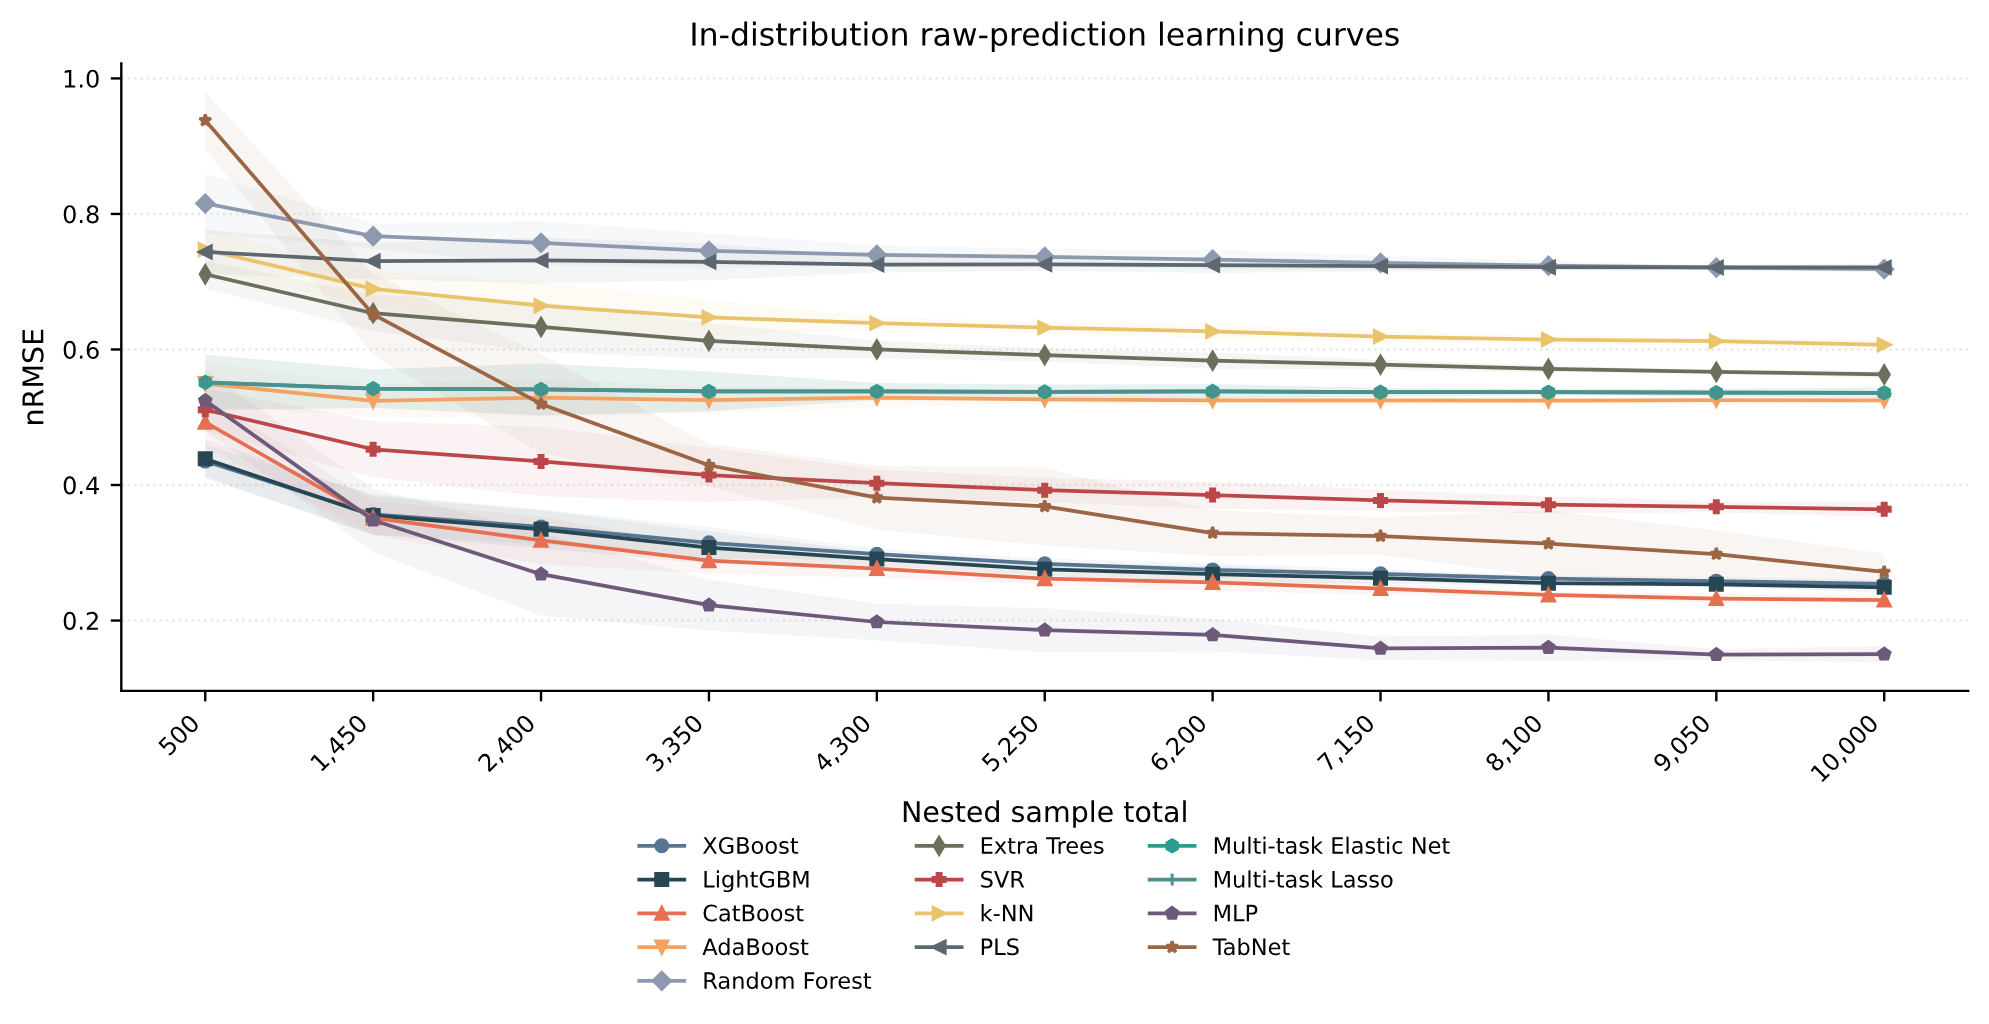
\includegraphics[width=0.96\textwidth]{main_figure_learning_curves.png}
\caption{In-distribution learning curves for raw predictions. Lines show five-fold mean nRMSE and shaded regions show $\pm$ one sample SD across folds.}
\label{fig:learning_curves}
\end{figure}

\subsection{Mass-Conservation and Non-Negativity Enforcement Effects}

Every raw prediction set violated the declared mass-conservation tolerance for every surrogate and data size. This result includes AdaBoost, Random Forest, Extra Trees, and $k$-NN, whose raw predictions were non-negative at $N=10{,}000$ (Table~\ref{tab:projection_physics}). Their positivity is expected for methods that average or select positive training responses: random forests aggregate tree predictions, $k$-NN uses neighboring responses, and averaging-type smoothers preserve positivity when the contributing responses are positive (Belkin et al., 2019; Breiman, 2001; Mack, 1981). That same operation does not preserve the case-specific affine balance, because the contributing responses come from different influent states; unconstrained data-driven models can therefore remain accurate while violating conservation laws (Kashinath et al., 2021; Sturm \& Wexler, 2020, 2022). For the remaining surrogates, raw non-negativity violations affected 39.0--76.8\% of validation rows at $N=10{,}000$, showing the complementary failure mode of accurate but unconstrained component regressions.

Projection eliminated both mass-conservation and non-negativity violations in all 750,750 in-distribution predictions. The maximum projected conservation residual was $2.06\times10^{-13}$, and no projected concentration was negative. This is the central structural result: after projection, every heterogeneous surrogate delivered a state that satisfied the same conservation and componentwise non-negativity requirements as the mechanistic benchmark, without changing how the surrogate was trained.

\FloatBarrier
\begin{table}[H]
\centering
\caption{Mass-conservation and non-negativity diagnostics at $N=10{,}000$. Raw rates and displacement are five-fold means. Every projected mass-conservation and non-negativity violation rate was zero.}
\label{tab:projection_physics}
\scriptsize
\resizebox{\textwidth}{!}{%
\begin{tabular}{lrrrrr}
\toprule
Surrogate & Raw mass violation (\%) & Raw non-negativity violation (\%) & Maximum projected $v_{mc}$ & Backtracking (\%) & Mean $d_c^{\mathrm{std}}$ \\
\midrule
XGBoost & 100.0 & 39.7 & $1.54\times10^{-13}$ & 0.00 & 0.300 \\
LightGBM & 100.0 & 39.0 & $1.61\times10^{-13}$ & 0.00 & 0.301 \\
CatBoost & 100.0 & 59.1 & $1.67\times10^{-13}$ & 0.00 & 0.242 \\
AdaBoost & 100.0 & 0.0 & $1.47\times10^{-13}$ & 0.30 & 0.901 \\
Random Forest & 100.0 & 0.0 & $1.73\times10^{-13}$ & 1.42 & 2.002 \\
Extra Trees & 100.0 & 0.0 & $1.72\times10^{-13}$ & 0.88 & 1.528 \\
SVR & 100.0 & 76.8 & $1.58\times10^{-13}$ & 0.01 & 0.363 \\
$k$-NN & 100.0 & 0.0 & $1.62\times10^{-13}$ & 0.25 & 1.192 \\
PLS & 100.0 & 54.3 & $1.47\times10^{-13}$ & 0.93 & 1.808 \\
Multi-task Elastic Net & 100.0 & 71.1 & $1.56\times10^{-13}$ & 0.00 & 0.482 \\
Multi-task Lasso & 100.0 & 71.0 & $1.72\times10^{-13}$ & 0.00 & 0.482 \\
MLP & 100.0 & 58.6 & $1.74\times10^{-13}$ & 0.00 & 0.189 \\
TabNet & 100.0 & 60.5 & $1.46\times10^{-13}$ & 0.04 & 0.545 \\
\bottomrule
\end{tabular}}
\end{table}
\FloatBarrier

Figure~\ref{fig:violation_trajectories} separates violation frequency from predictive error. The raw mass-conservation rate was identically 100\%, and both projected rates were identically zero, at all eleven sizes. The raw non-negativity trajectories differed. CatBoost increased from 12.8\% at $N=500$ to 59.1\% at $N=10{,}000$, XGBoost from 33.4\% to 39.7\%, and SVR from 68.4\% to 76.8\%. LightGBM decreased and then partially rebounded, MLP decreased from 86.4\% to 58.6\%, and TabNet was non-monotonic. These patterns show why conservation and non-negativity must be diagnosed separately from nRMSE: as a surrogate learns the response surface more closely, it can still cross a zero boundary in a small component or miss a conserved invariant by a small but systematic amount. This separation is consistent with prior physical machine learning studies in which high conventional accuracy coexisted with violations of conservation or positivity (Hansen et al., 2024; Kashinath et al., 2021; Kircher \& Votsmeier, 2025; Sturm \& Silva, 2024).

The rising non-negativity incidence for some high-accuracy surrogates is not evidence that additional data degraded their global fit. A row is counted when any one of 20 outputs crosses zero, and the events were concentrated in low-valued $S_A$, $S_{NH4}$, $S_{NO2}$, $S_{NO3}$, and $X_{PHA}$ states. Symmetric regression losses and independently or jointly unconstrained output layers contain no barrier at zero; non-negative outputs require explicit constraints, transformations, or positivity-preserving corrections (Kircher \& Votsmeier, 2025; Lakshminarayanan et al., 2017; Sturm \& Wexler, 2022). Resolving these near-boundary tails can therefore lower nRMSE while allowing more small negative undershoots. For SVR, for example, the violation rate increased while its mean standardized negative magnitude fell from 0.271 to 0.222 and raw nRMSE fell from 0.511 to 0.364. Violation frequency and severity must consequently be interpreted separately, and the useful effect of projection is that both are reduced to zero while the conservation residual is simultaneously controlled.

\begin{figure}[htbp]
\centering
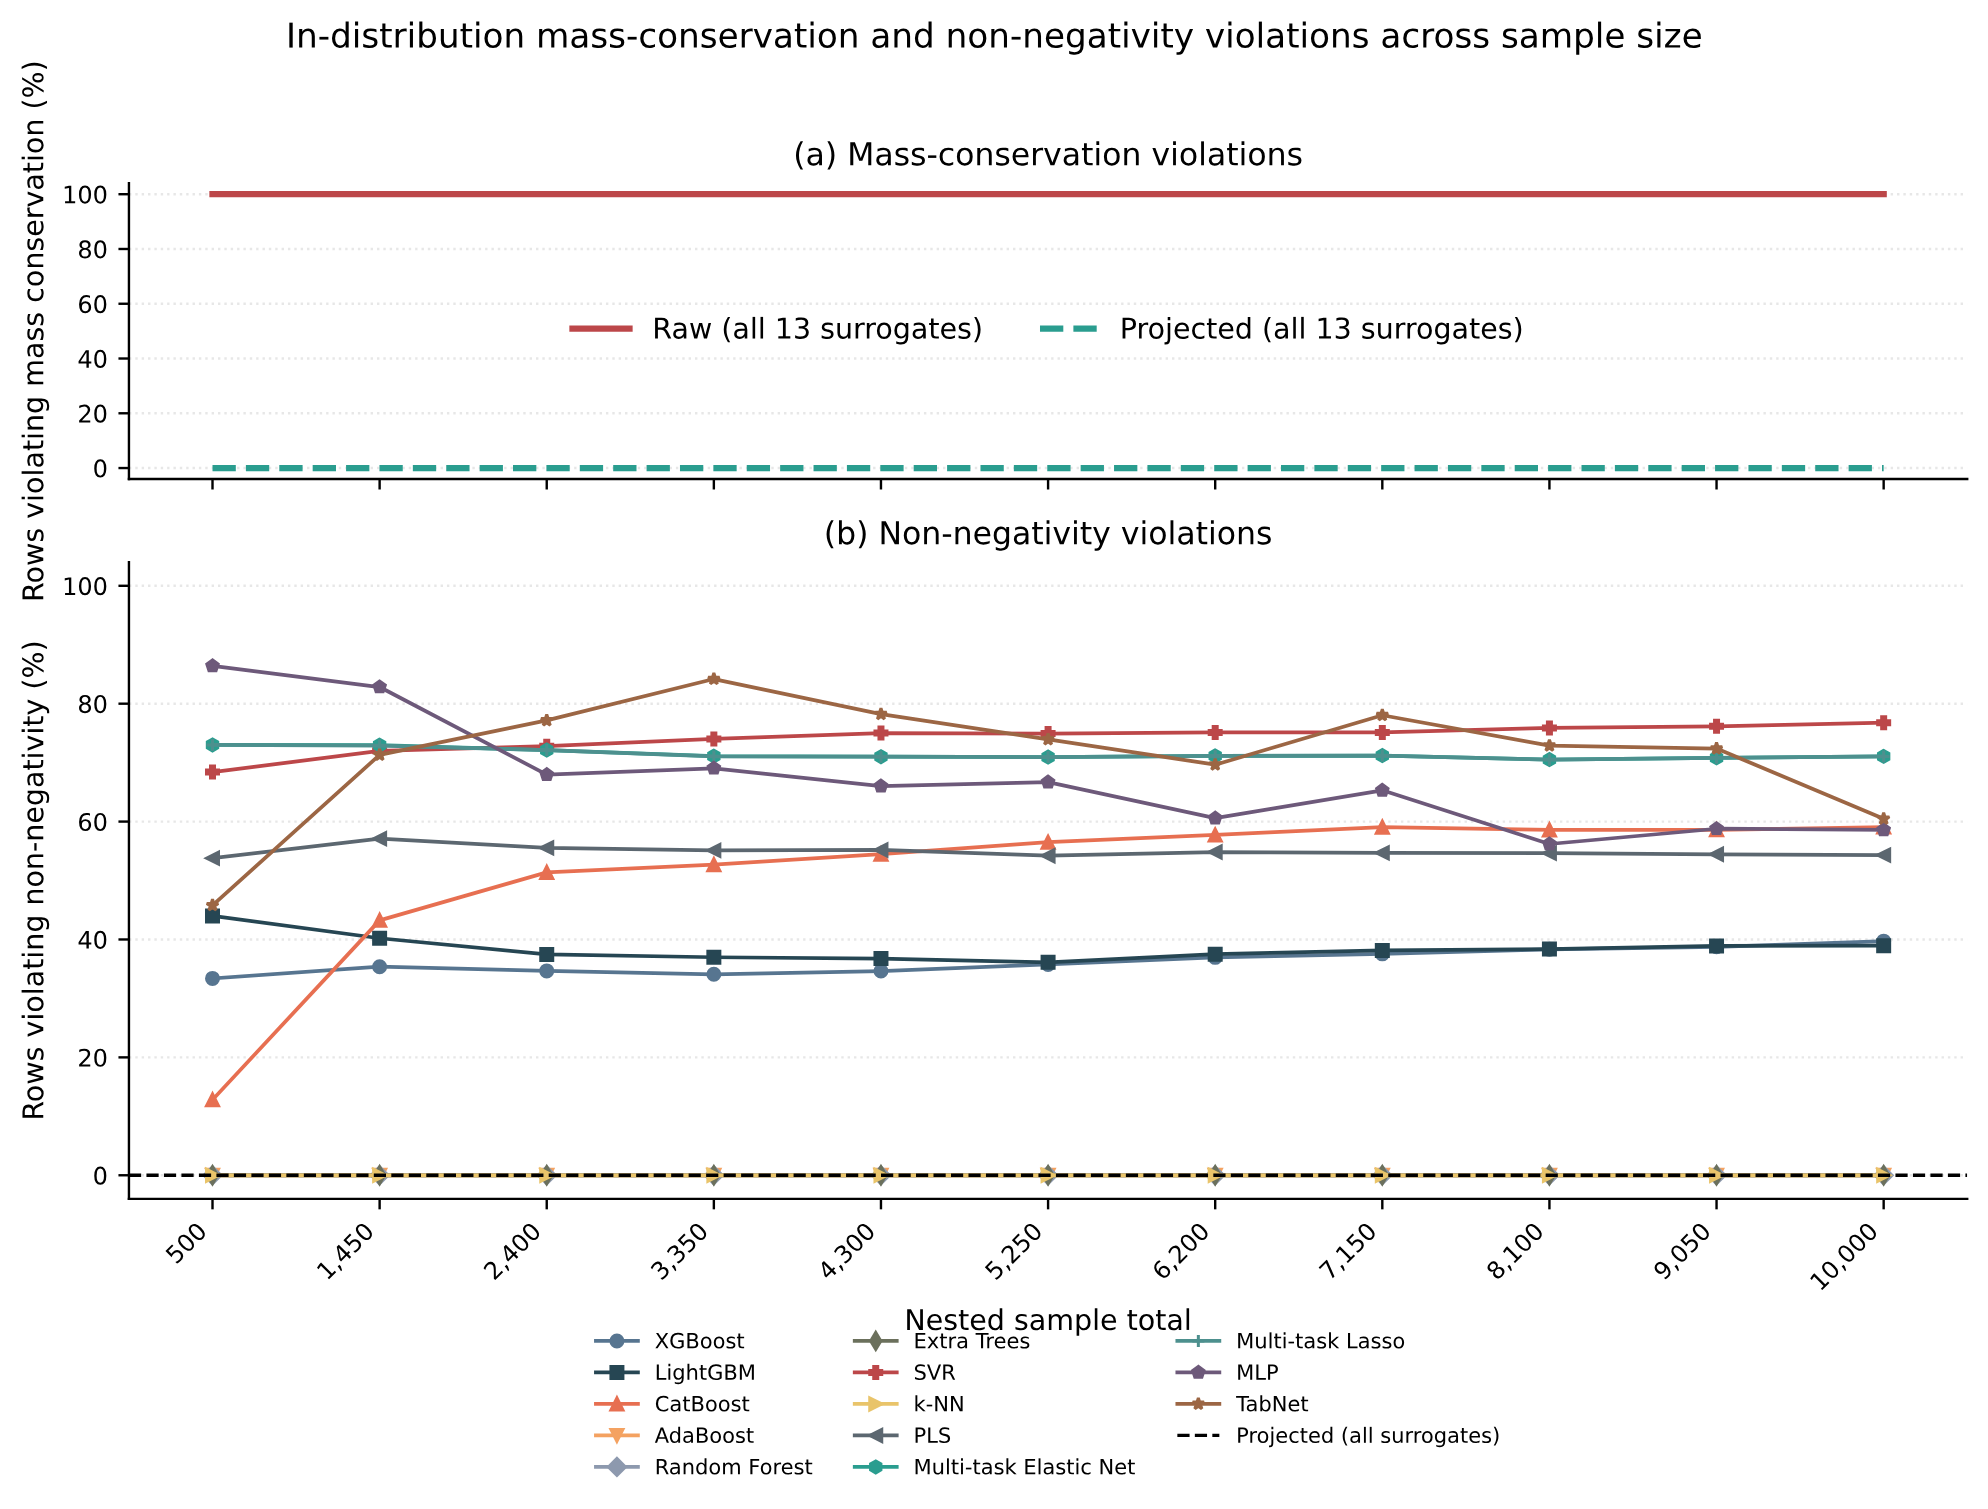
\includegraphics[width=0.96\textwidth]{main_figure_violation_rates_by_sample_size.png}
\caption{In-distribution mass-conservation and non-negativity violation rates across nested sample totals. Curves are five-fold means. All 13 raw mass-conservation curves coincide at 100\%, all projected mass-conservation and non-negativity curves coincide at 0\%, and the remaining curves show raw non-negativity violations.}
\label{fig:violation_trajectories}
\end{figure}

\begin{figure}[htbp]
\centering
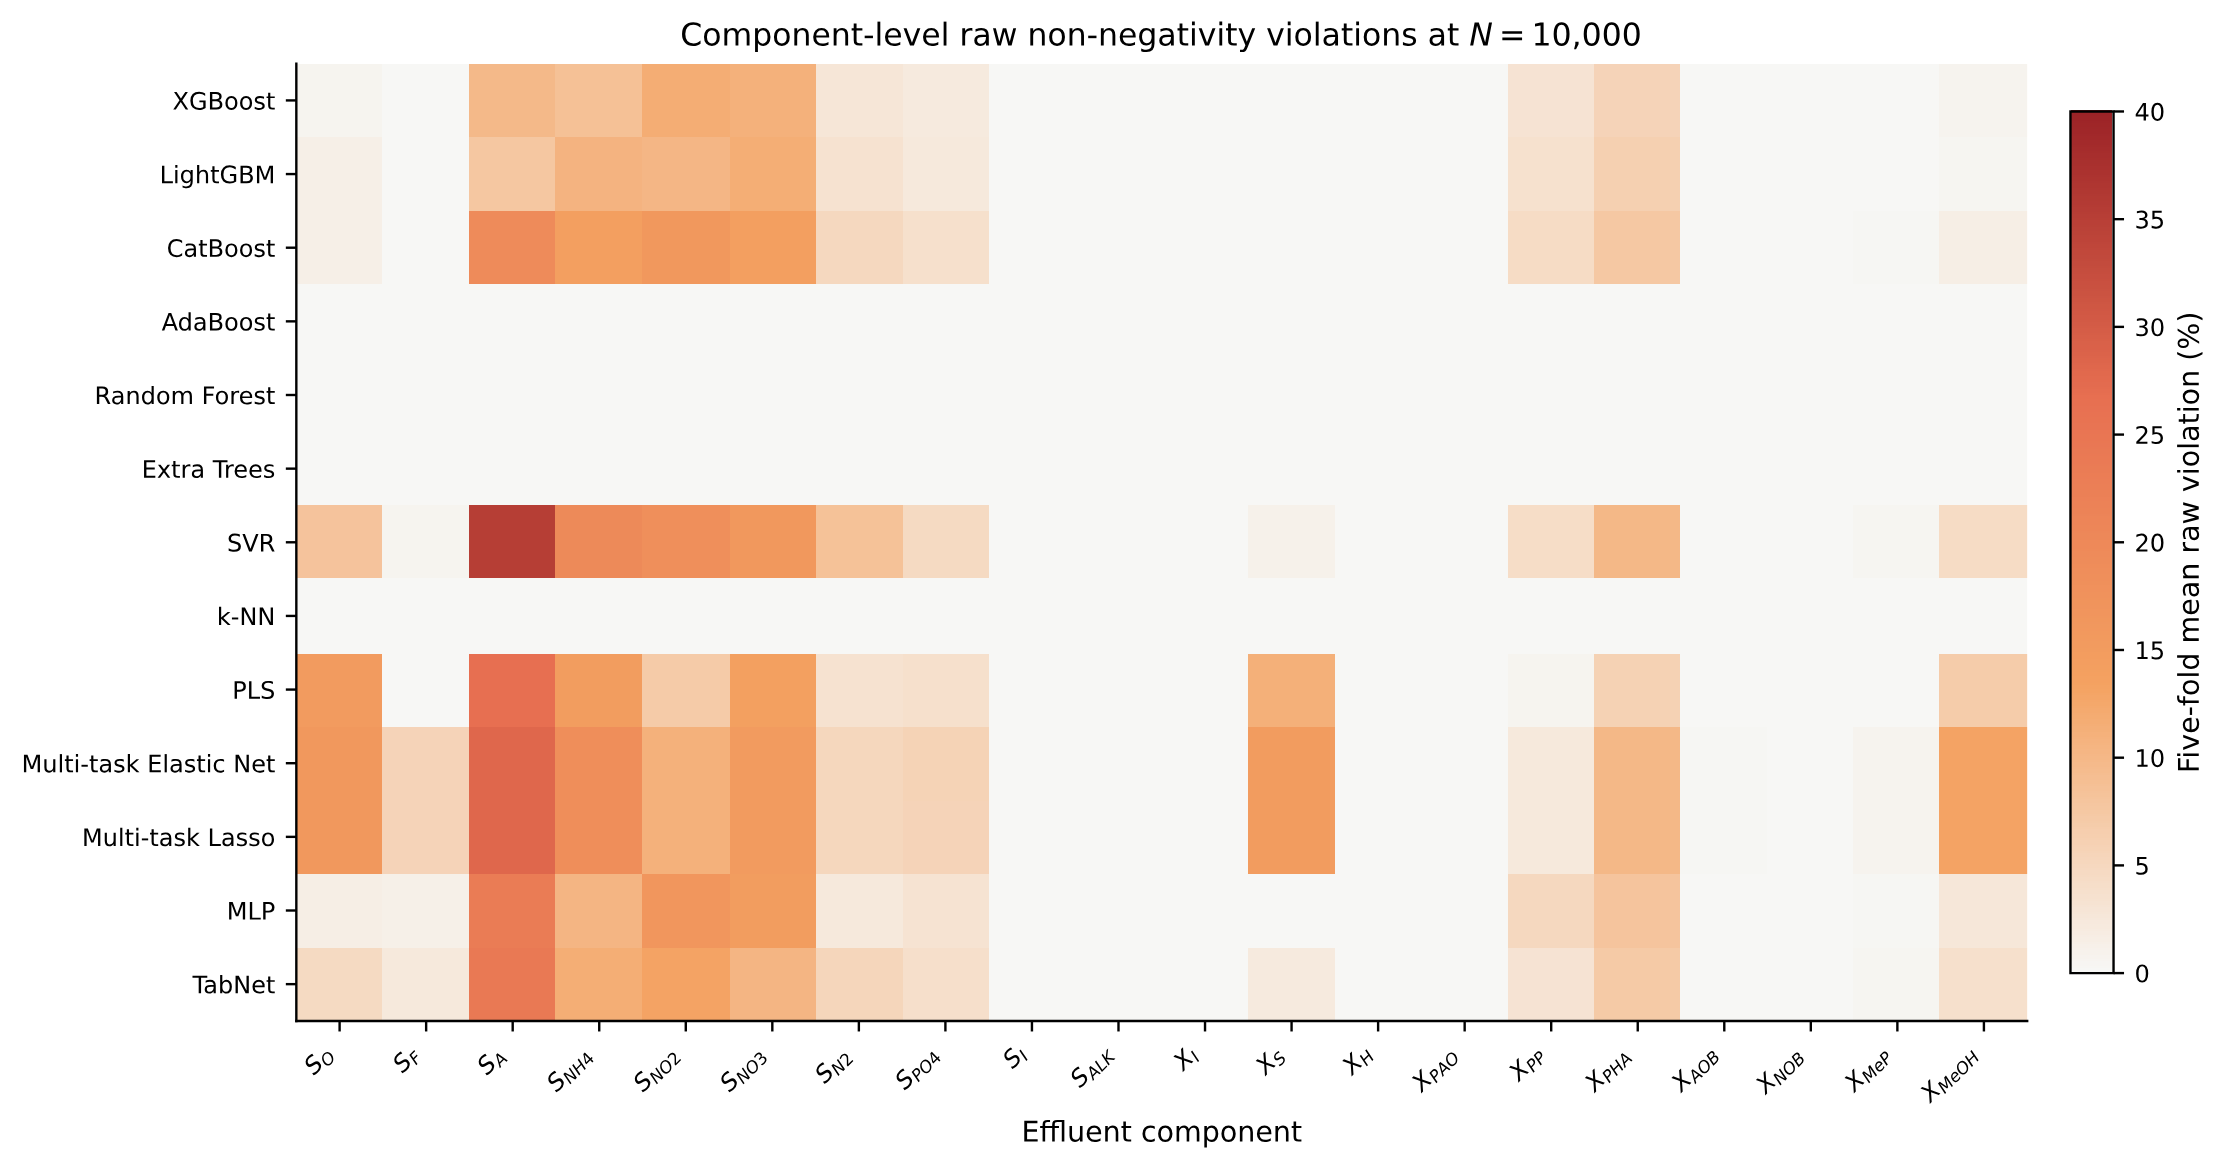
\includegraphics[width=0.98\textwidth]{main_figure_component_nonnegativity_violations_id.png}
\caption{Component-level raw non-negativity violations at $N=10{,}000$. Rows are surrogates and columns are effluent components. Each cell is the five-fold mean percentage of validation predictions in which that component was below the declared non-negativity tolerance. Projected values are not shown because every projected component had a 0\% violation rate.}
\label{fig:component_nonnegativity_violations}
\end{figure}

Figure~\ref{fig:component_nonnegativity_violations} localizes the row-level rates in Table~\ref{tab:projection_physics}. AdaBoost, Random Forest, Extra Trees, and $k$-NN had zero violations for all 20 components. Among the remaining surrogates, violations were concentrated in a subset of low-valued components. Across all 13 surrogates, $S_A$ had the highest mean component-level rate (15.5\%) and reached 35.1\% for SVR; $S_{NH4}$, $S_{NO3}$, and $S_{NO2}$ followed at 9.7\%, 9.3\%, and 8.8\%, respectively. No raw violation occurred in $S_{ALK}$, $X_I$, or $X_H$. Thus, the row-level percentages reflect recurring boundary crossings in particular outputs rather than uniform negativity across the component vector. Any such crossing still makes the raw state inadmissible, while projection reduced every surrogate--component cell to zero. The concentration of violations in small nitrogen and substrate pools is also consistent with the aggregate accuracy results: the best surrogates were close enough overall that their infeasible values were often near-boundary artifacts rather than broad failures of process prediction.

The accuracy effect in Figure~\ref{fig:projection_change} was governed by how each surrogate's error aligned with the feasible affine space and by the standardized weighting and positivity backtracking, rather than by surrogate family alone. Multi-task Elastic Net and Multi-task Lasso benefited at all eleven sizes and in all five full-size folds. Their joint linear fits can retain systematic cross-component residuals outside the conservation subspace; because the mechanistic target lies inside that subspace, projection removes a repeatable error direction. Neither surrogate required positivity backtracking, so this reconciliation was not diluted by a subsequent move toward the influent anchor. PLS shows why linearity alone is insufficient: it improved 16 of 20 component nRMSE values, but its larger displacement and backtracking-induced $S_F$ and $X_H$ losses produced a $+0.024$ aggregate nRMSE cost.

SVR changed from projection costs at $N=1{,}450$--4,300 to benefits at every size from $N=5{,}250$ onward. Once its unconstrained component regressors learned the within-manifold response more accurately, reconciliation removed a larger fraction of the remaining cross-component inconsistency. The boosting surrogates showed a related movement toward neutrality: the mean projection cost over their first four sizes versus their last four sizes declined from 0.0264 to 0.0030 for CatBoost, from 0.0174 to 0.0006 for XGBoost, and from 0.0063 to 0.0004 for LightGBM as projection displacement also contracted. CatBoost crossed into a small benefit at $N=8{,}100$ and 10,000, whereas XGBoost and LightGBM remained slightly adverse in aggregate. MLP and TabNet alternated signs rather than showing a monotonic trend; MLP improved by 0.0016 at full size, while TabNet worsened by 0.0032. Thus, when a raw surrogate is already accurate, projection often changes nRMSE only marginally while changing mass-conservation and non-negativity compliance from universally failed to universally satisfied. In activated sludge use, low predictive error without both mass conservation and non-negativity is not sufficient evidence that a predicted state is physically usable, because the process state must remain compatible with component mass balances and physically meaningful non-negative concentrations (Araujo et al., 2013; Kircher \& Votsmeier, 2025).

\begin{figure}[htbp]
\centering
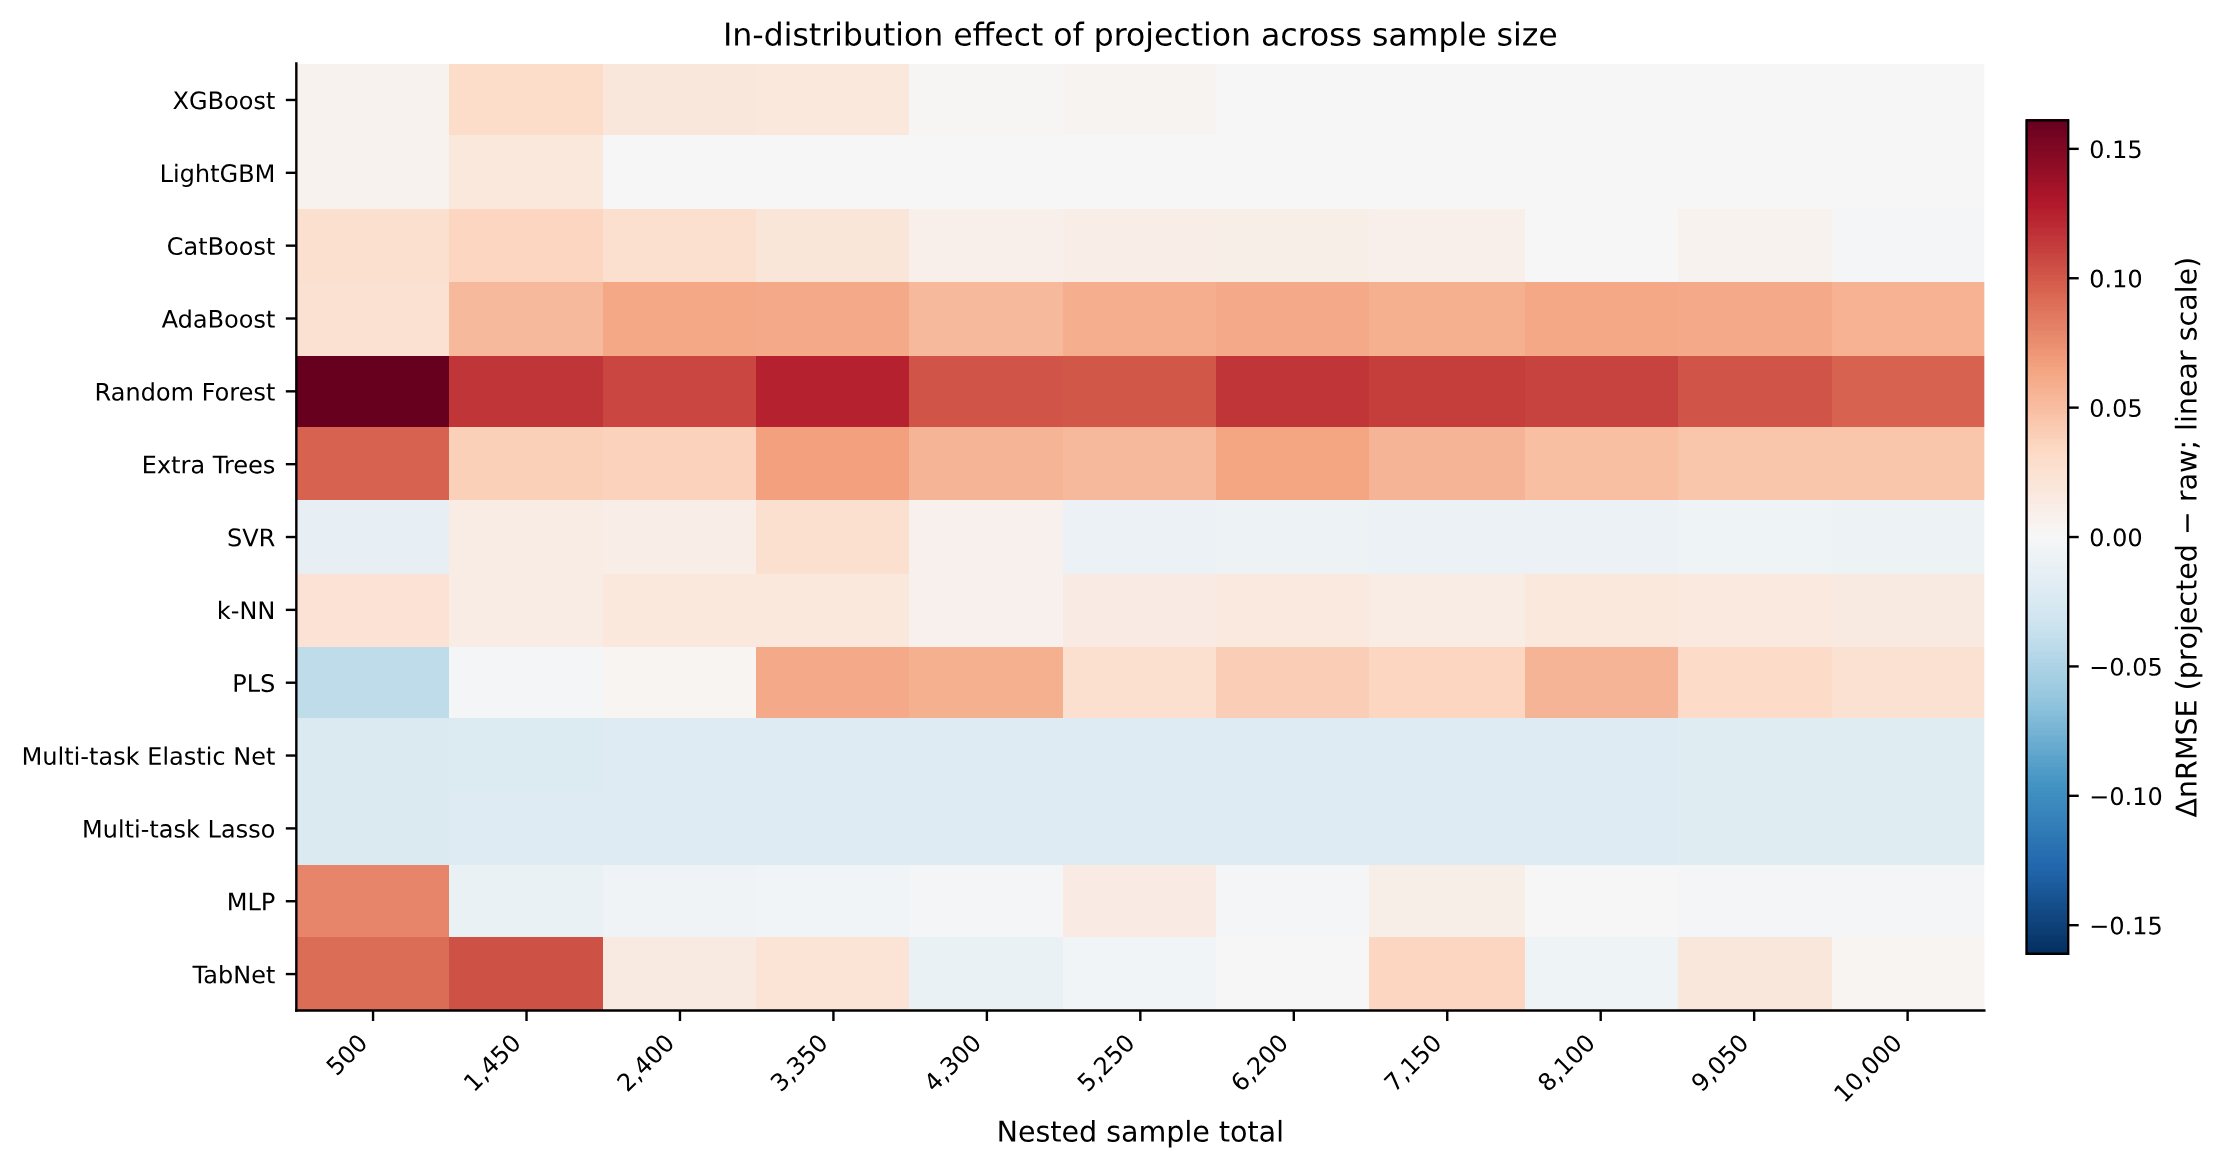
\includegraphics[width=0.94\textwidth]{main_figure_projection_change.png}
\caption{Change in in-distribution nRMSE after projection for every surrogate and nested sample total. Each cell is projected minus raw five-fold mean nRMSE; negative values indicate lower error after projection.}
\label{fig:projection_change}
\end{figure}

Component-level results explain why counts of improved outputs and aggregate nRMSE can disagree (Figure~\ref{fig:id_component_projection_effects}). Projection lowered mean component nRMSE in 188 of 260 surrogate--component pairs (72.3\%) and for a majority of components in 12 of 13 surrogates; AdaBoost was the exception at 9 of 20. Multi-task Elastic Net and Multi-task Lasso improved 18 components each, MLP 17, and CatBoost, PLS, and SVR 16. All 13 surrogates improved $S_I$, $S_{ALK}$, $X_{MeP}$, $S_{PO4}$, $X_{MeOH}$, $S_{N2}$, $S_{NO2}$, and $X_{NOB}$, but $X_H$ worsened for every surrogate. These patterns show that the projection usually moved the prediction in a physically useful direction across the component vector, while the squared aggregate metric could still be dominated by a small number of larger adverse movements.

The two largest recurring losses have different explanations. Effluent $S_F$ was small and right-skewed (mean 2.22 and median 1.45 g COD m$^{-3}$), but its column in $A$ was numerically null. The conservative projection therefore left $S_F$ essentially unchanged unless positivity backtracking shortened the entire influent-to-candidate direction. That shared shortening can pull $S_F$ toward an influent concentration near 100 g COD m$^{-3}$. For Random Forest at full size, the $S_F$ mean squared error was unchanged on the 9,858 non-backtracked predictions, while the 142 backtracked predictions accounted for its increase from component nRMSE 0.887 to 1.993. By contrast, $X_H$ was not a small component: its mean was 187.1 g COD m$^{-3}$. The inverse-concentration weights penalize relative rather than absolute movement, making a large component such as $X_H$ comparatively inexpensive to move in physical units; the resulting correction was frequently misaligned with the $X_H$ target and introduced a negative bias. Supplementary Tables~S2 and S3 show the full cross-analysis. All surrogates improved TN and TP composite nRMSE, whereas all worsened COD and TSS; the near-elimination of TP error is consistent with the TP composition vector's near-alignment with the phosphorus invariant.

\begin{figure}[htbp]
\centering
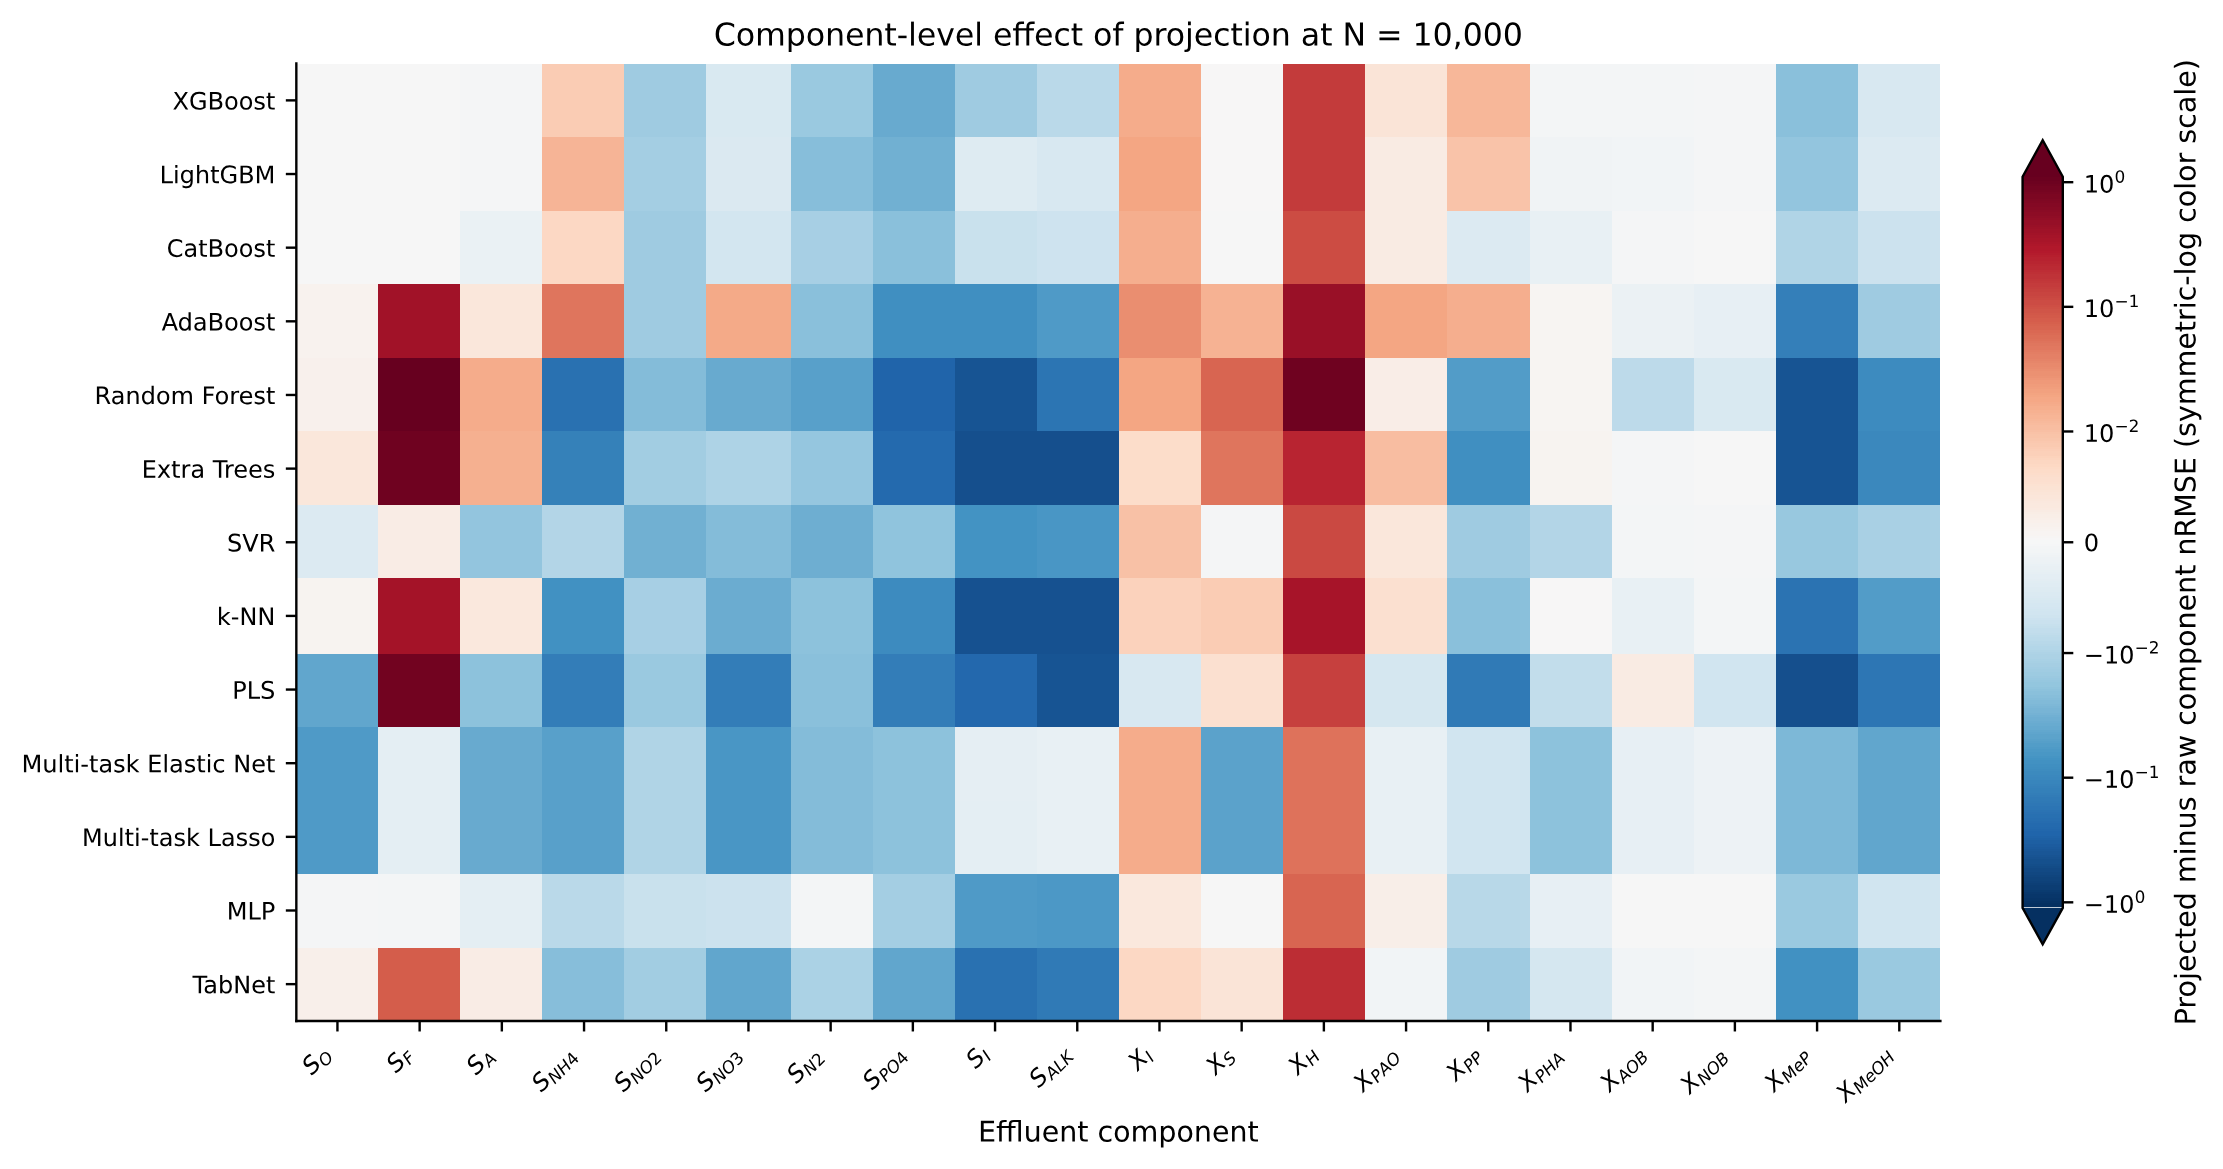
\includegraphics[width=0.98\textwidth]{main_figure_component_projection_effects_id.png}
\caption{Component-level change in in-distribution nRMSE at $N=10{,}000$. Each cell is the mean of five paired fold differences (projected minus raw); blue denotes lower error and red denotes higher error. The symmetric-log color scale displays small and large changes without clipping.}
\label{fig:id_component_projection_effects}
\end{figure}

Positivity backtracking was required for 2,489 of the 750,750 in-distribution projections (0.332\%). Random Forest (904), PLS (574), and Extra Trees (566) accounted for 82.1\% of these activations and also had among the largest full-size standardized displacements (2.002, 1.808, and 1.528). Their provisional conservative corrections were therefore more likely to cross the non-negative orthant boundary, at which point a common scalar shortened the entire direction toward the feasible influent anchor. This explains both the concentration of backtracking and its ability to affect components that do not directly participate in the five invariants. The low activation rate also clarifies why the projection was primarily a conservation reconciliation step for most predictions, with positivity backtracking acting as a targeted safeguard for the small fraction of cases whose conservative correction would otherwise leave the non-negative orthant. Complete surrogate-specific counts are given in Supplementary Table~S4.

\subsection{Extrapolation Beyond the Training Domain}

Error increased from mild to severe extrapolation for every raw and projected surrogate (Table~\ref{tab:ood_accuracy}). This monotonic increase confirms that the exterior inputs formed a harder predictive problem than interpolation within the training envelope, consistent with the broader limitation that data-driven models usually generalize less reliably under distribution shift or outside their training support (Karniadakis et al., 2021; Shen et al., 2023; Valente et al., 2025). MLP retained the lowest observed nRMSE in both regimes, followed by TabNet, matching the full-size in-distribution pattern that favored neural surrogates when enough training data were available. Projection reduced aggregate nRMSE in 11 of 13 mild-regime comparisons and 9 of 13 severe-regime comparisons. The exceptions were AdaBoost and Random Forest in both regimes, plus Extra Trees and $k$-NN under severe extrapolation.

The larger out-of-distribution benefit is consistent with the interpretation developed in-distribution: when extrapolation increases cross-component inconsistency, projecting the 20-component vector back to the feasible invariant balance can remove a larger share of the residual error. Projection and hard-constrained correction methods have been used for exactly this purpose: moving model outputs onto physically consistent constraint sets so that infeasible residual components are removed or controlled (Hansen et al., 2024; Sturm \& Silva, 2024; Valente et al., 2025). At the same time, the tree and neighbor exceptions show that non-negative averaging-based surrogates can require sizeable corrections when they are asked to extrapolate, and those corrections can increase aggregate nRMSE even while restoring physical admissibility. This trade-off is consistent with constrained-learning studies showing that enforcing physical consistency can change standard error metrics, particularly outside the range where a purely data-driven model is reliable (Shen et al., 2023; Sturm \& Silva, 2024; Valente et al., 2025).

\FloatBarrier
\begin{table}[H]
\centering
\caption{Out-of-distribution nRMSE for full-data surrogate refits. Each value summarizes 600 separately simulated cases.}
\label{tab:ood_accuracy}
\scriptsize
\begin{tabular}{lrrrr}
\toprule
Surrogate & Mild raw & Mild projected & Severe raw & Severe projected \\
\midrule
XGBoost & 0.424 & 0.420 & 0.861 & 0.853 \\
LightGBM & 0.419 & 0.413 & 0.848 & 0.842 \\
CatBoost & 0.393 & 0.387 & 0.836 & 0.828 \\
AdaBoost & 0.692 & 0.711 & 1.036 & 1.139 \\
Random Forest & 0.908 & 0.996 & 1.242 & 1.489 \\
Extra Trees & 0.717 & 0.679 & 1.084 & 1.222 \\
SVR & 0.555 & 0.538 & 0.989 & 0.948 \\
$k$-NN & 0.760 & 0.732 & 1.113 & 1.147 \\
PLS & 0.908 & 0.841 & 1.267 & 1.190 \\
Multi-task Elastic Net & 0.750 & 0.688 & 1.146 & 1.044 \\
Multi-task Lasso & 0.751 & 0.688 & 1.146 & 1.044 \\
MLP & 0.255 & 0.251 & 0.531 & 0.521 \\
TabNet & 0.336 & 0.333 & 0.563 & 0.547 \\
\bottomrule
\end{tabular}
\end{table}
\FloatBarrier

Aggregate improvements again coexisted with opposing component effects (Figure~\ref{fig:ood_component_projection_effects}). Projection reduced component nRMSE in 192 of 260 mild comparisons (73.8\%) and 193 of 260 severe comparisons (74.2\%). Every surrogate improved a majority of its components in both regimes. Multi-task Elastic Net and Multi-task Lasso improved 18 of 20 components under mild and 19 under severe extrapolation, while SVR increased from 12 mild improvements to 18 severe improvements. The principal adverse cells were again $X_H$ and, for the tree ensembles, AdaBoost, and $k$-NN, $S_F$; under severe extrapolation, Random Forest worsened by 1.965 nRMSE units for $X_H$ and 1.238 for $S_F$. The repetition of the same adverse components across in-distribution and out-of-distribution evaluation links the extrapolation behavior to the projection geometry rather than to a new failure mode: $S_F$ is weakly controlled by the invariant operator, while $X_H$ can absorb relatively large physical movements under inverse-concentration weighting. Supplementary Tables~S6--S9 provide every raw, projected, and paired-change component and composite value for both regimes.

\begin{figure}[htbp]
\centering
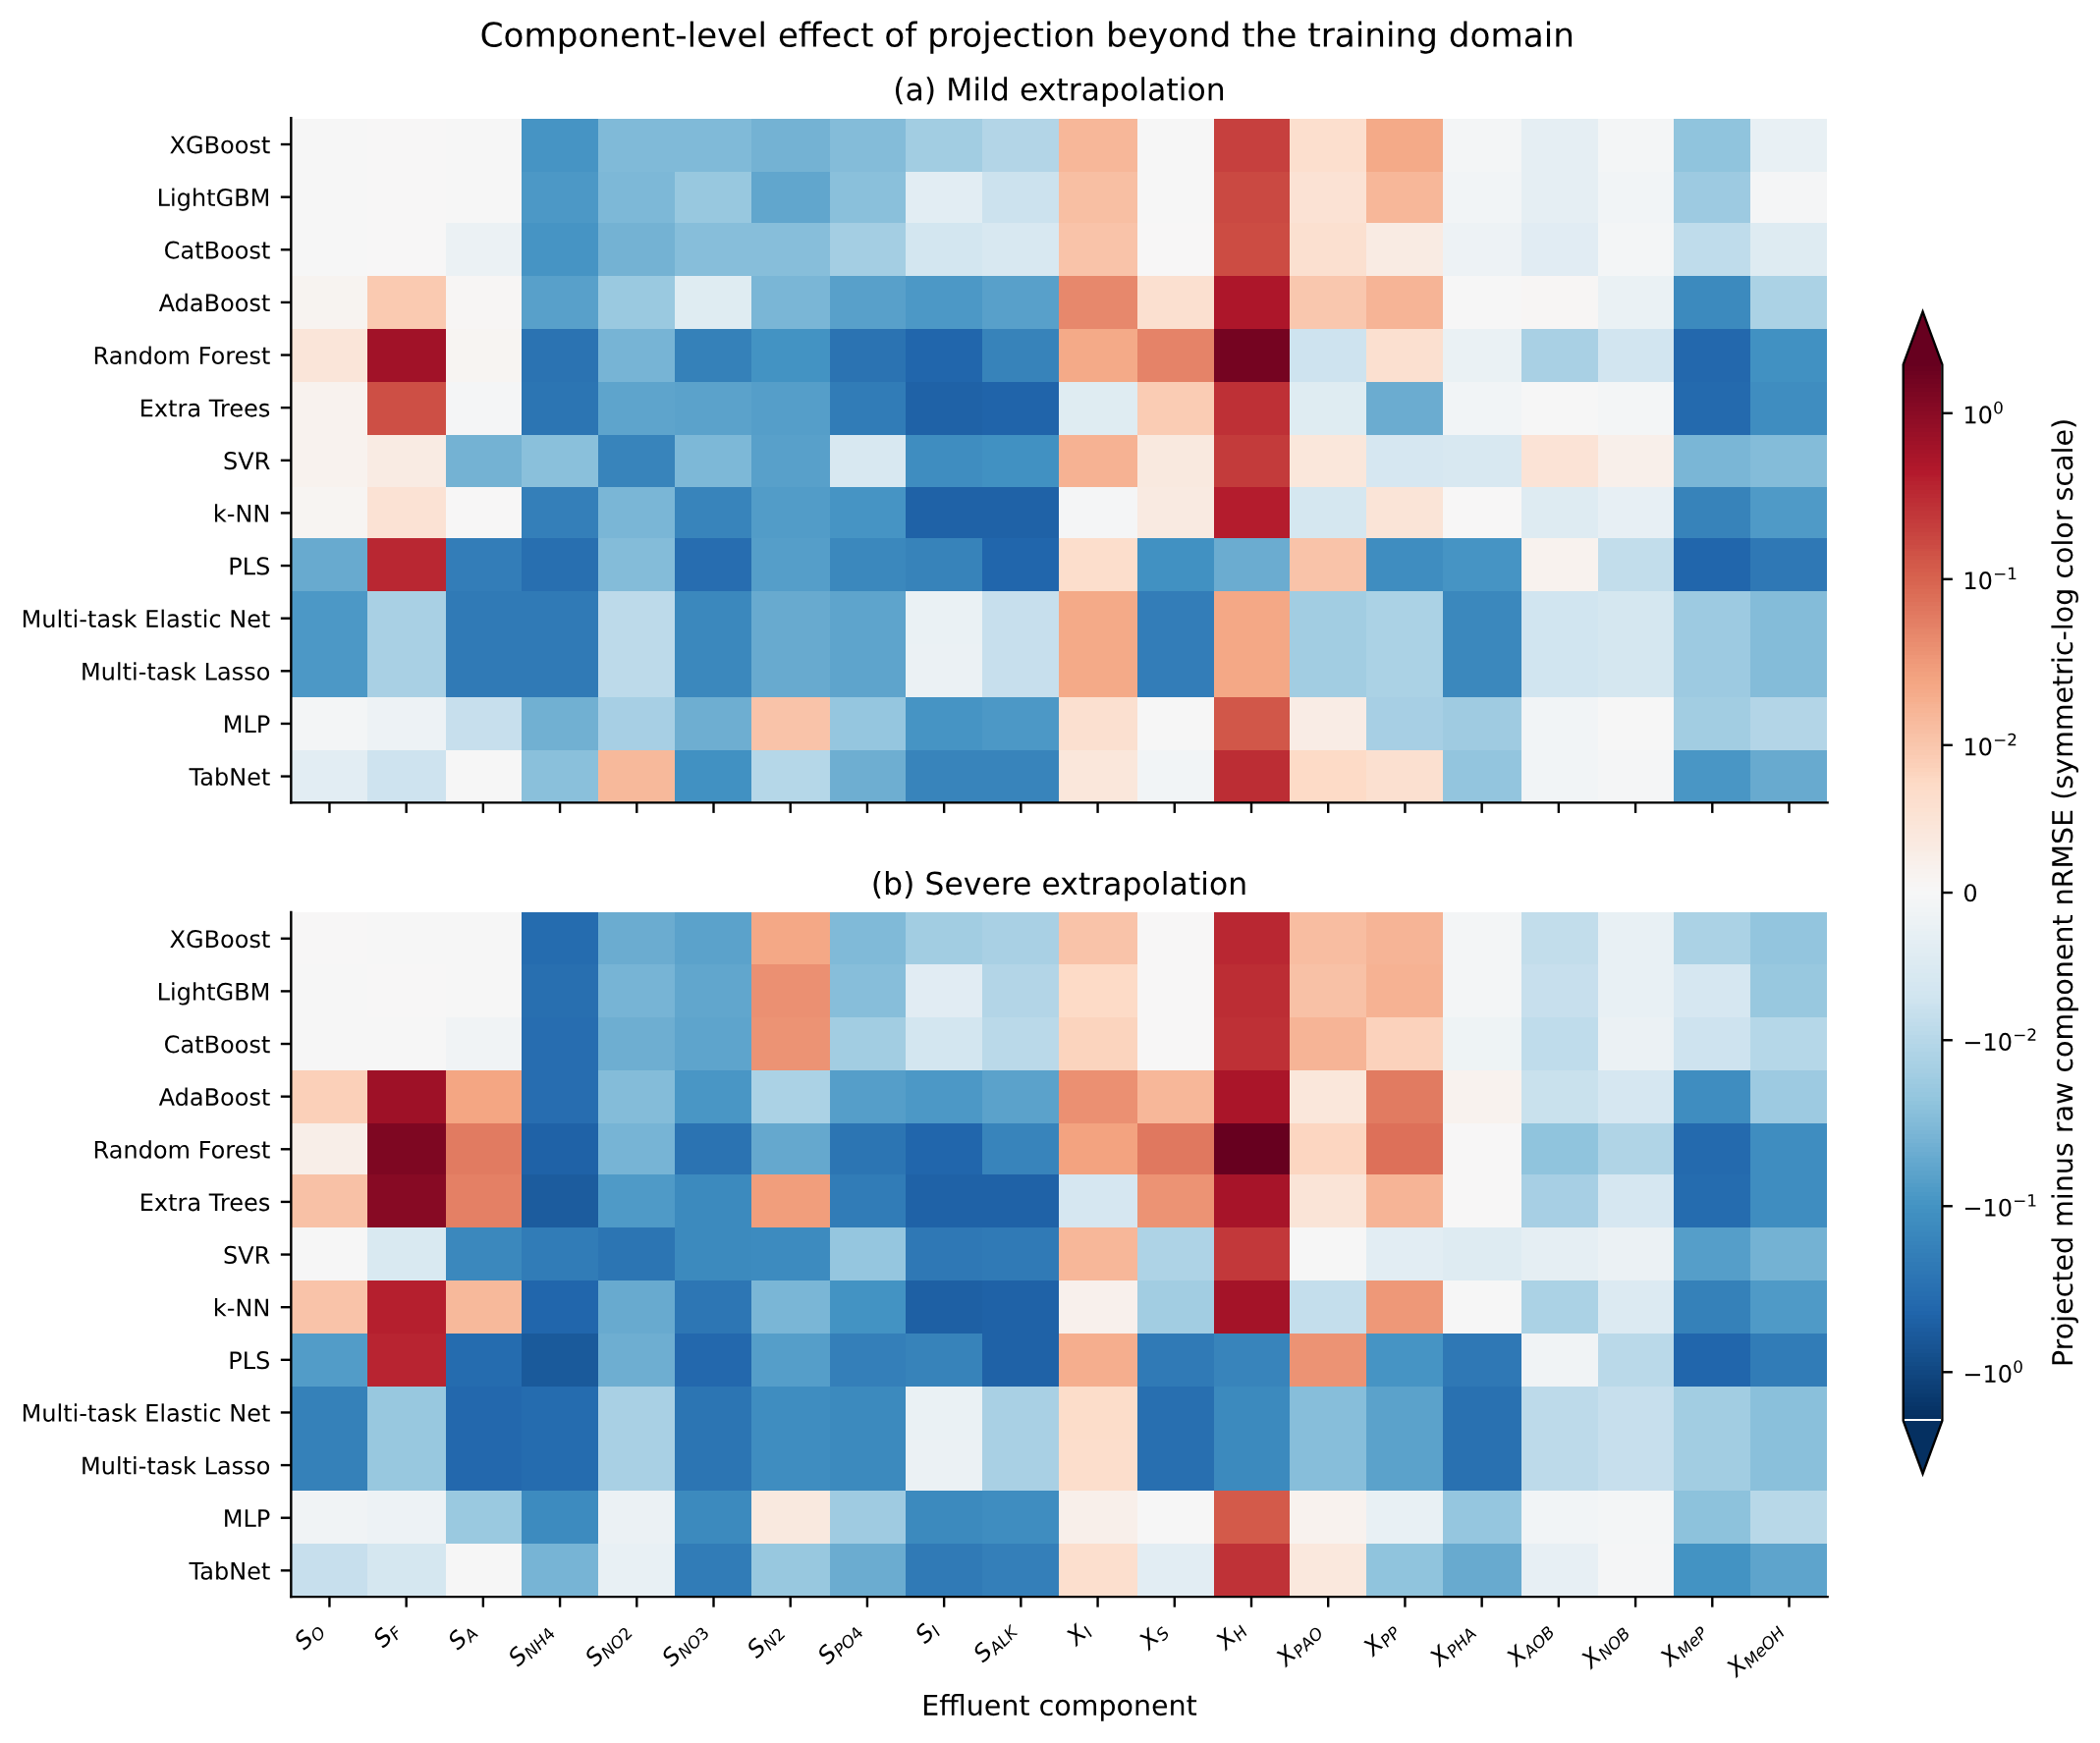
\includegraphics[width=0.98\textwidth]{main_figure_ood_component_projection_effects.png}
\caption{Component-level change in nRMSE after projection for mild and severe extrapolation. Each cell uses the same 600 mechanistic cases before and after projection; blue denotes lower error and red denotes higher error. The common symmetric-log color scale permits direct comparison without clipping.}
\label{fig:ood_component_projection_effects}
\end{figure}

Every raw out-of-distribution prediction set violated mass conservation. Projection produced zero mass-conservation and non-negativity violations across all 15,600 out-of-distribution surrogate predictions, with a maximum projected conservation residual of $1.72\times10^{-13}$. Backtracking was activated for 68 predictions (0.436\%). Together with the 750,750 in-distribution projected predictions, this gives 766,350 evaluated projected predictions, all of which satisfied the enforced physical requirements. This establishes the main overall conclusion: projection is a reliable feasibility safeguard across surrogate families and data domains, while the predictive-error change reflects how each surrogate's residuals are distributed across the feasible and infeasible directions. The evidence here is based on simulated steady states, so the enforced guarantees should be interpreted specifically as mass-conservation and non-negativity guarantees for the evaluated activated sludge component vectors. Within that scope, the practical implication is strong: projection prevents accurate but physically inadmissible raw predictions from entering downstream interpretation, optimization, or control. This matters because wastewater and process-system surrogates are increasingly used in design, operation, and decision-support workflows, where downstream choices depend on predictions that remain physically interpretable (Durkin et al., 2024; Mao et al., 2024; Shen et al., 2023; Tang et al., 2026; Yang et al., 2021).

\FloatBarrier
\section{Conclusion}

Fast statistical surrogates are attractive because they can replace repeated activated sludge simulations with much cheaper predictions. The risk is that a prediction can look close to the simulated answer while still breaking the physical bookkeeping that gives the state meaning. In this work, the two non-negotiable checks were simple to state: the predicted effluent had to conserve the declared mass-balance invariants, and none of its 20 component concentrations could be negative. The results show that these checks are not optional add-ons to ordinary error metrics. They answer a different question: not only whether a prediction is close, but whether it can be treated as a physically admissible activated sludge state at all.

The study tested this distinction across a deliberately broad set of surrogates and data conditions. Thirteen statistical surrogates were trained and evaluated across eleven in-distribution sample sizes, from scarce data to the full $N=10{,}000$ benchmark, and then tested again on two separately simulated extrapolation regimes. The Kircher--Votsmeier projection was applied only after each surrogate had already predicted the full 20-component effluent vector. It therefore did not require a custom model architecture, a special loss function, or retraining. This is important for practice: the same feasibility layer was tested on boosting surrogates, random ensembles, kernel and neighbor methods, linear and latent-variable surrogates, and neural networks.

The central finding is clear. Every raw surrogate prediction set violated mass conservation, even when the same model produced low predictive error and even when all of its raw concentrations were non-negative. Several accurate raw surrogates also predicted negative values in small components. After projection, these failures disappeared. All $750{,}750$ in-distribution projected predictions and all $15{,}600$ out-of-distribution projected predictions conserved mass and remained non-negative. The largest projected conservation residuals were only $2.06\times10^{-13}$ in-distribution and $1.72\times10^{-13}$ out-of-distribution. In plain terms, the projection turned every evaluated surrogate output into a state that obeyed the two enforced physical requirements.

The accuracy story was more nuanced, and that nuance is one of the useful lessons of the work. Projection was not an automatic error reducer. At the largest in-distribution sample size, it reduced aggregate nRMSE for five surrogates and increased it for eight. Outside the training range, however, it reduced aggregate nRMSE in 20 of 26 surrogate--regime comparisons. At the component level, the effect was more often favorable: projection lowered nRMSE in 188 of 260 in-distribution surrogate--component comparisons, 192 of 260 mild-extrapolation comparisons, and 193 of 260 severe-extrapolation comparisons. These numbers show why aggregate accuracy alone can hide the main behavior. Projection often moved many individual components in a better and more physically meaningful direction, while a few larger adverse movements could still dominate the aggregate score.

The model comparisons also reinforce a practical message. MLP had the lowest observed full-size in-distribution and out-of-distribution errors, TabNet improved strongly as the dataset grew, and boosted trees were especially competitive under smaller training sets. Yet none of these accuracy differences removed the need for physical checks. The projection worked as a common safeguard across all surrogate families, while its effect on predictive error depended on how each surrogate's residuals lined up with the feasible mass-balance space and with the non-negative concentration boundary.

The implication is that wastewater surrogate evaluation should separate two questions that are often blended together. First, is the prediction accurate enough for the intended use? Second, is the prediction physically admissible enough to be interpreted, optimized, or passed into downstream decision tools? This work addresses the second question directly. Within the simulated steady-state benchmark studied here, post-prediction projection provided a reliable way to enforce mass conservation and non-negativity without changing the underlying surrogate. That guarantee should not be overread as proof of kinetic realism, field performance, or universal process validity. It is narrower, but valuable: it prevents accurate-looking yet physically impossible predictions from being treated as usable activated sludge states.

\section*{CRediT authorship contribution statement}

The sole author, E.F.S.J., contributed to conceptualization, methodology, software, validation, formal analysis, investigation, resources, data curation, writing---original draft, writing---review \& editing, visualization, supervision, project administration, and funding acquisition.

\section*{Acknowledgments \& disclosure of funding}

This work is funded by the Department of Science and Technology of the Philippines through the Engineering Research and Development for Technology scholarship awarded to the sole author, E.F.S.J., at the University of San Carlos.

\section*{Data availability}

The complete codebase that reproduces the results presented in this study is available in the GitHub repository \texttt{https://github.com/egbertoselerio1997/surrogate-projection.git}. The repository may be cloned using the command \texttt{git clone https://github.com/egbertoselerio1997/surrogate-projection.git}.

\section*{References}

\noindent Aboagye, E. A., Burnham, S. M., Dailey, J., Zia, R., Tran, C., Desai, M., \& Yenkie, K. M. (2021). Systematic design, optimization, and sustainability assessment for generation of efficient wastewater treatment networks. \textit{Water, 13}(9), 1326. doi: 10.3390/w13091326.

\noindent Araujo, A. C. B. de, Gallani, S., Mulas, M., \& Skogestad, S. (2013). Sensitivity analysis of optimal operation of an activated sludge process model for economic controlled variable selection. \textit{Industrial \& Engineering Chemistry Research, 52}(29), 9908--9921. doi: 10.1021/ie4006673.

\noindent Argyriou, A., Evgeniou, T., \& Pontil, M. (2008). Convex multi-task feature learning. \textit{Machine Learning, 73}(3), 243--272. doi: 10.1007/s10994-007-5040-8.

\noindent Arik, S. \"O., \& Pfister, T. (2021). TabNet: Attentive interpretable tabular learning. \textit{Proceedings of the AAAI Conference on Artificial Intelligence, 35}(8), 6679--6687. doi: 10.1609/aaai.v35i8.16826.

\noindent Belkin, M., Hsu, D., Ma, S., \& Mandal, S. (2019). Reconciling modern machine-learning practice and the classical bias-variance trade-off. \textit{Proceedings of the National Academy of Sciences, 116}(32), 15849--15854. doi: 10.1073/pnas.1903070116.

\noindent Beucler, T., Pritchard, M., Rasp, S., Ott, J., Baldi, P., \& Gentine, P. (2021). Enforcing analytic constraints in neural networks emulating physical systems. \textit{Physical Review Letters, 126}(9), 098302. doi: 10.1103/PhysRevLett.126.098302.

\noindent Bhosekar, A., \& Ierapetritou, M. (2018). Advances in surrogate based modeling, feasibility analysis, and optimization: A review. \textit{Computers \& Chemical Engineering, 108}, 250--267. doi: 10.1016/j.compchemeng.2017.09.017.

\noindent Borisov, V., Leemann, T., Sessler, K., Haug, J., Pawelczyk, M., \& Kasneci, G. (2024). Deep neural networks and tabular data: A survey. \textit{IEEE Transactions on Neural Networks and Learning Systems, 35}(6), 7499--7519. doi: 10.1109/TNNLS.2022.3229161.

\noindent Breiman, L. (2001). Random forests. \textit{Machine Learning, 45}(1), 5--32. doi: 10.1023/A:1010933404324.

\noindent Chen, T., \& Guestrin, C. (2016). XGBoost: A scalable tree boosting system. In \textit{Proceedings of the 22nd ACM SIGKDD International Conference on Knowledge Discovery and Data Mining} (pp. 785--794). Association for Computing Machinery. doi: 10.1145/2939672.2939785.

\noindent Curteanu, S., \& Cartwright, H. (2011). Neural networks applied in chemistry. I. Determination of the optimal topology of multilayer perceptron neural networks. \textit{Journal of Chemometrics, 25}(10), 527--548. doi: 10.1002/cem.1401.

\noindent Drucker, H. (1997). Improving regressors using boosting techniques. In D. H. Fisher (Ed.), \textit{Proceedings of the Fourteenth International Conference on Machine Learning} (pp. 107--115). Morgan Kaufmann.

\noindent Duan, S., Zhang, Y., \& Zheng, S. (2022). Heterotrophic nitrifying bacteria in wastewater biological nitrogen removal systems: A review. \textit{Critical Reviews in Environmental Science and Technology, 52}(13), 2302--2338. doi: 10.1080/10643389.2021.1877976.

\noindent Durkin, A., Otte, L., \& Guo, M. (2024). Surrogate-based optimisation of process systems to recover resources from wastewater. \textit{Computers \& Chemical Engineering, 182}, 108584. doi: 10.1016/j.compchemeng.2024.108584.

\noindent Geurts, P., Ernst, D., \& Wehenkel, L. (2006). Extremely randomized trees. \textit{Machine Learning, 63}(1), 3--42. doi: 10.1007/s10994-006-6226-1.

\noindent Guerrero, J., Guisasola, A., \& Baeza, J. A. (2011). The nature of the carbon source rules the competition between PAO and denitrifiers in systems for simultaneous biological nitrogen and phosphorus removal. \textit{Water Research, 45}(16), 4793--4802. doi: 10.1016/j.watres.2011.06.019.

\noindent Hansen, D., Maddix, D. C., Alizadeh, S., Gupta, G., \& Mahoney, M. W. (2024). Learning physical models that can respect conservation laws. \textit{Physica D: Nonlinear Phenomena, 457}, 133952. doi: 10.1016/j.physd.2023.133952.

\noindent Henze, M., Gujer, W., Mino, T., \& van Loosdrecht, M. (2006). Activated Sludge Models ASM1, ASM2, ASM2d and ASM3. \textit{Water Intelligence Online, 5}(0). doi: 10.2166/9781780402369.

\noindent Hornik, K., Stinchcombe, M., \& White, H. (1989). Multilayer feedforward networks are universal approximators. \textit{Neural Networks, 2}(5), 359--366. doi: 10.1016/0893-6080(89)90020-8.

\noindent Karniadakis, G. E., Kevrekidis, I. G., Lu, L., Perdikaris, P., Wang, S., \& Yang, L. (2021). Physics-informed machine learning. \textit{Nature Reviews Physics, 3}(6), 422--440. doi: 10.1038/s42254-021-00314-5.

\noindent Kashinath, K., Mustafa, M., Albert, A., Wu, J. L., Jiang, C., Esmaeilzadeh, S., Azizzadenesheli, K., Wang, R., Chattopadhyay, A., Singh, A., Manepalli, A., Chirila, D., Yu, R., Walters, R., White, B., Xiao, H., Tchelepi, H. A., Marcus, P., Anandkumar, A., \& Prabhat. (2021). Physics-informed machine learning: Case studies for weather and climate modelling. \textit{Philosophical Transactions of the Royal Society A: Mathematical, Physical and Engineering Sciences, 379}(2194), 20200093. doi: 10.1098/rsta.2020.0093.

\noindent Ke, G., Meng, Q., Finley, T., Wang, T., Chen, W., Ma, W., Ye, Q., \& Liu, T.-Y. (2017). LightGBM: A highly efficient gradient boosting decision tree. In \textit{Advances in Neural Information Processing Systems} (Vol. 30, pp. 3146--3154). Curran Associates, Inc.

\noindent Kircher, T., \& Votsmeier, M. (2025). Machine learning surrogate models for mechanistic kinetics: Embedding atom balance and positivity. \textit{The Journal of Physical Chemistry Letters, 16}(19), 4715--4723. doi: 10.1021/acs.jpclett.5c00602.

\noindent Lakshminarayanan, B., Pritzel, A., \& Blundell, C. (2017). Simple and scalable predictive uncertainty estimation using deep ensembles. In \textit{Advances in Neural Information Processing Systems} (Vol. 30, pp. 6402--6413). Curran Associates, Inc.

\noindent Lin, L., Yang, H., \& Xu, X. (2022). Effects of water pollution on human health and disease heterogeneity: A review. \textit{Frontiers in Environmental Science, 10}, 880246. doi: 10.3389/fenvs.2022.880246.

\noindent Liu, H., Palatucci, M., \& Zhang, J. (2009). Blockwise coordinate descent procedures for the multi-task lasso, with applications to neural semantic basis discovery. In \textit{Proceedings of the 26th Annual International Conference on Machine Learning} (pp. 649--656). Association for Computing Machinery. doi: 10.1145/1553374.1553458.

\noindent Mack, Y. P. (1981). Local properties of $k$-NN regression estimates. \textit{SIAM Journal on Algebraic Discrete Methods, 2}(3), 311--323. doi: 10.1137/0602035.

\noindent Madhav, S., Ahamad, A., Singh, A. K., Kushawaha, J., Chauhan, J. S., Sharma, S., \& Singh, P. (2019). Water pollutants: Sources and impact on the environment and human health. In \textit{Sensors in water pollutants monitoring: Role of material} (pp. 43--62). doi: 10.1007/978-981-15-0671-0\_4.

\noindent Mao, Z., Li, X., Zhang, X., Li, D., Lu, J., Li, J., \& Zheng, F. (2024). Optimization of effluent quality and energy consumption of aeration process in wastewater treatment plants using artificial intelligence. \textit{Journal of Water Process Engineering, 63}, 105384. doi: 10.1016/j.jwpe.2024.105384.

\noindent Min, Y., Sonar, A., \& Azizan, N. (2024). HardNet: Hard-constrained neural networks with universal approximation guarantees. \textit{arXiv preprint arXiv:2410.10807}.

\noindent Padron-Paez, J. I., Almaraz, S. D. L., \& Rom\'an-Mart\'inez, A. (2020). Sustainable wastewater treatment plants design through multiobjective optimization. \textit{Computers \& Chemical Engineering, 140}, 106850. doi: 10.1016/j.compchemeng.2020.106850.

\noindent Prokhorenkova, L., Gusev, G., Vorobev, A., Dorogush, A. V., \& Gulin, A. (2018). CatBoost: Unbiased boosting with categorical features. In \textit{Advances in Neural Information Processing Systems} (Vol. 31, pp. 6638--6648). Curran Associates, Inc.

\noindent Raissi, M., Perdikaris, P., \& Karniadakis, G. E. (2019). Physics-informed neural networks: A deep learning framework for solving forward and inverse problems involving nonlinear partial differential equations. \textit{Journal of Computational Physics, 378}, 686--707. doi: 10.1016/j.jcp.2018.10.045.

\noindent Rumelhart, D. E., Hinton, G. E., \& Williams, R. J. (1986). Learning representations by back-propagating errors. \textit{Nature, 323}(6088), 533--536. doi: 10.1038/323533a0.

\noindent Simon, N., Friedman, J., \& Hastie, T. (2013). A blockwise descent algorithm for group-penalized multiresponse and multinomial regression. \textit{arXiv preprint arXiv:1311.6529}. doi: 10.48550/arXiv.1311.6529.

\noindent Shen, C., Appling, A. P., Gentine, P., Bandai, T., Gupta, H. V., Tartakovsky, A., Baity-Jesi, M., Hill, N., Chen, K., \& Ji, X. (2023). Differentiable modeling to unify machine learning and physical models and advance geosciences. \textit{Nature Reviews Earth \& Environment, 4}, 209--228. doi: 10.1038/s43017-023-00450-9.

\noindent Shwartz-Ziv, R., \& Armon, A. (2022). Tabular data: Deep learning is not all you need. \textit{Information Fusion, 81}, 84--90. doi: 10.1016/j.inffus.2021.11.011.

\noindent Smola, A. J., \& Sch\"olkopf, B. (2004). A tutorial on support vector regression. \textit{Statistics and Computing, 14}(3), 199--222. doi: 10.1023/B:STCO.0000035301.49549.88.

\noindent Sturm, P. M., Cappa, C. D., \& Wexler, A. S. (2023). Advecting superspecies: Efficiently modeling transport of organic aerosol with a mass-conserving dimensionality reduction method. \textit{Journal of Advances in Modeling Earth Systems, 15}(3), e2022MS003235. doi: 10.1029/2022MS003235.

\noindent Sturm, P. O., \& Silva, S. J. (2024). A nudge to the truth: Atom conservation as a hard constraint in models of atmospheric composition using a species-weighted correction. \textit{ACS ES\&T Air, 2}(1), 99--108. doi: 10.1021/acsestair.4c00220.

\noindent Sturm, P. M., \& Wexler, A. S. (2020). A mass- and energy-conserving framework for using machine learning to speed computations: A photochemistry example. \textit{Geoscientific Model Development, 13}(9), 4435--4442. doi: 10.5194/gmd-13-4435-2020.

\noindent Sturm, P. M., \& Wexler, A. S. (2022). Conservation laws in a neural network architecture: Enforcing the atom balance of a Julia-based photochemical model (v0.2.0). \textit{Geoscientific Model Development, 15}(9), 3417--3431. doi: 10.5194/gmd-15-3417-2022.

\noindent Tang, Y., Cui, T., Zhou, W., \& Chang, C. (2026). Surrogate model-based optimal design of coal chemical wastewater treatment networks with a multi-stage system. \textit{Processes, 14}(3), 806. doi: 10.3390/pr14050806.

\noindent Utkarsh, Maddix, D. C., Ma, R., Mahoney, M. W., \& Wang, Y. (2025). End-to-end probabilistic framework for learning with hard constraints. \textit{arXiv preprint arXiv:2506.07003}.

\noindent Valente, M., Dias, T. C., Guerra, V., \& Ventura, R. (2025). Physics-consistent machine learning with output projection onto physical manifolds. \textit{Communications Physics, 8}(1), 180. doi: 10.1038/s42005-025-02329-1.

\noindent Wang, Y., Li, T., Bai, L., Yu, H., \& Qu, F. (2025). Comparison of interpretable machine learning models and mechanistic model for predicting effluent nitrogen in WWTP. \textit{Journal of Water Process Engineering, 77}, 108344. doi: 10.1016/j.jwpe.2025.108344.

\noindent Wold, S., Sj\"ostr\"om, M., \& Eriksson, L. (2001). PLS-regression: A basic tool of chemometrics. \textit{Chemometrics and Intelligent Laboratory Systems, 58}(2), 109--130. doi: 10.1016/S0169-7439(01)00155-1.

\noindent Woo, S. H., Lee, D. S., \& Park, J. M. (2009). On-line estimation of key process variables based on kernel partial least squares in an industrial cokes wastewater treatment plant. \textit{Journal of Hazardous Materials, 161}(1), 538--544. doi: 10.1016/j.jhazmat.2008.04.004.

\noindent Xiao, Y., Zhao, B., Zhang, X., \& Yue, X. (2025). A new paradigm in activated sludge management: An interpretable framework integrating mechanistic dynamics with a data-driven surrogate model. \textit{Environmental Research}, 123435. doi: 10.1016/j.envres.2025.123435.

\noindent Yang, S. J., Kim, J., Eom, J., Kim, M., Lee, M., \& Lee, K. H. (2025). Machine learning based prediction of waste activated sludge generation for optimization of WWTP operational efficiency. \textit{Environmental Research}, 122990. doi: 10.1016/j.envres.2025.122990.

\noindent Yang, C., Zhang, Y., Huang, M., \& Liu, H. (2021). Adaptive dynamic prediction of effluent quality in wastewater treatment processes using partial least squares embedded with relevance vector machine. \textit{Journal of Cleaner Production, 314}, 128076. doi: 10.1016/j.jclepro.2021.128076.

\noindent Yuan, M., \& Lin, Y. (2006). Model selection and estimation in regression with grouped variables. \textit{Journal of the Royal Statistical Society: Series B (Statistical Methodology), 68}(1), 49--67. doi: 10.1111/j.1467-9868.2005.00532.x.

\noindent Zou, H., \& Hastie, T. (2005). Regularization and variable selection via the elastic net. \textit{Journal of the Royal Statistical Society: Series B (Statistical Methodology), 67}(2), 301--320. doi: 10.1111/j.1467-9868.2005.00503.x.

\end{document}
